%! TEX program = lualatex

%https://docs.google.com/presentation/d/1tzJUNB0fMNV5wQB0rjdc64slcNY_xHncZjPgyFm8huU/edit?usp=sharing

\documentclass[nobackground,dvipsnames,table]{beamer}
%\usepackage{sio}
\usepackage{tsc}
\usepackage{pdfpc}
\usepackage{pgfpages}
\usepackage{multimedia}

%%%%%%%% edit hyperlink colors %%%%%%%%
\hypersetup{
  colorlinks   = true, 
  urlcolor     = tscurl, % color of external hyperlinks
  linkcolor    = white,   % color of internal links
}

%%%%% the below command allows custom highlights used in this presentation with \hlc %%%%%%
\newcommand{\hlc}[2][yellow]{{%
    \colorlet{foo}{#1}%
    \sethlcolor{foo}\hl{#2}}%
}   
%%%%%%%%%%%%%%%%%%%%%%%%%%%%%%%%%%%%%%%%%%%

%%% below command addresses log output error when trying to use \\ in \author %%%
\pdfstringdefDisableCommands{%
  \def\\{}%
}

\mode<presentation>
{\usetheme{default}
	\usecolortheme{tsc}
	\setbeamercovered{transparent}
	\useinnertheme[shadow=false]{rounded}
	\usebackgroundtemplate{}
	\setbeamercolor*{frametitle}{parent=palette primary}
	\setbeamerfont{block title}{size={}}
	\setbeamertemplate{navigation symbols}{}
    \setbeamertemplate{itemize items}[circle]
        \setbeamertemplate{enumerate items}[circle]
}
%{\usetheme{Hannover}
%	\usecolortheme{sio}
%	\setbeamercovered{transparent}
%	\useinnertheme[shadow=false]{rounded}
%	\usebackgroundtemplate{}
%	\setbeamercolor*{frametitle}{parent=palette primary}
%	\setbeamerfont{block title}{size={}}
%	\setbeamertemplate{navigation symbols}{}
%}

%%%%%%%%%%%%%%%%%%%%%%%%%%%%%%%%%%%%%%%%%%%%%%%%
%%%%%%%%%%%%%%%%  SLIDE 1  %%%%%%%%%%%%%%%%%%%%%
%%%%%%%%%%%%%%%%%%%%%%%%%%%%%%%%%%%%%%%%%%%%%%%%
\title[Content Moderation]{Content Moderation}
%\subtitle{A document made with thought and care}

\author[Seering]{Joseph Seering (KAIST)}
%\institute[SIO]{\large Stanford Internet Observatory}
\date[]{}
\subject{Trust and Safety}
\AddToShipoutPictureBG*{
  \AtPageLowerLeft{\hspace{-0.4cm}
    
\includegraphics[width=13.1cm]{img/consortium-image}}
}

% Change this to make a file with just slides, just notes or both
%\setbeameroption{hide notes}                 % Only slides
%\setbeameroption{show only notes}            % Only notes
\setbeameroption{show notes on second screen} % Both

\begin{document}

%\coverpage

\begin{frame}
	\titlepage
\end{frame}

%%%%%%%%%%%%%%%%%%%%%%%%%%%%%%%%%%%%%%%%%%%%%%%%
%%%%%%%%%%%%%%%%  SLIDE 2  %%%%%%%%%%%%%%%%%%%%%
%%%%%%%%%%%%%%%%%%%%%%%%%%%%%%%%%%%%%%%%%%%%%%%%
\begin{frame}{Learning objectives}
Today we will:

\begin{itemize}
    \item Begin to understand the breadth of models for content moderation
    \item Learn how to conceptualize different approaches to moderating a space.
    \item Reflect on how these models could evolve in the future
\end{itemize}
\end{frame}

%%%%%%%%%%%%%%%%%%%%%%%%%%%%%%%%%%%%%%%%%%%%%%%%
%%%%%%%%%%%%%%%%  SLIDE 3  %%%%%%%%%%%%%%%%%%%%%
%%%%%%%%%%%%%%%%%%%%%%%%%%%%%%%%%%%%%%%%%%%%%%%%
\begin{frame}{}

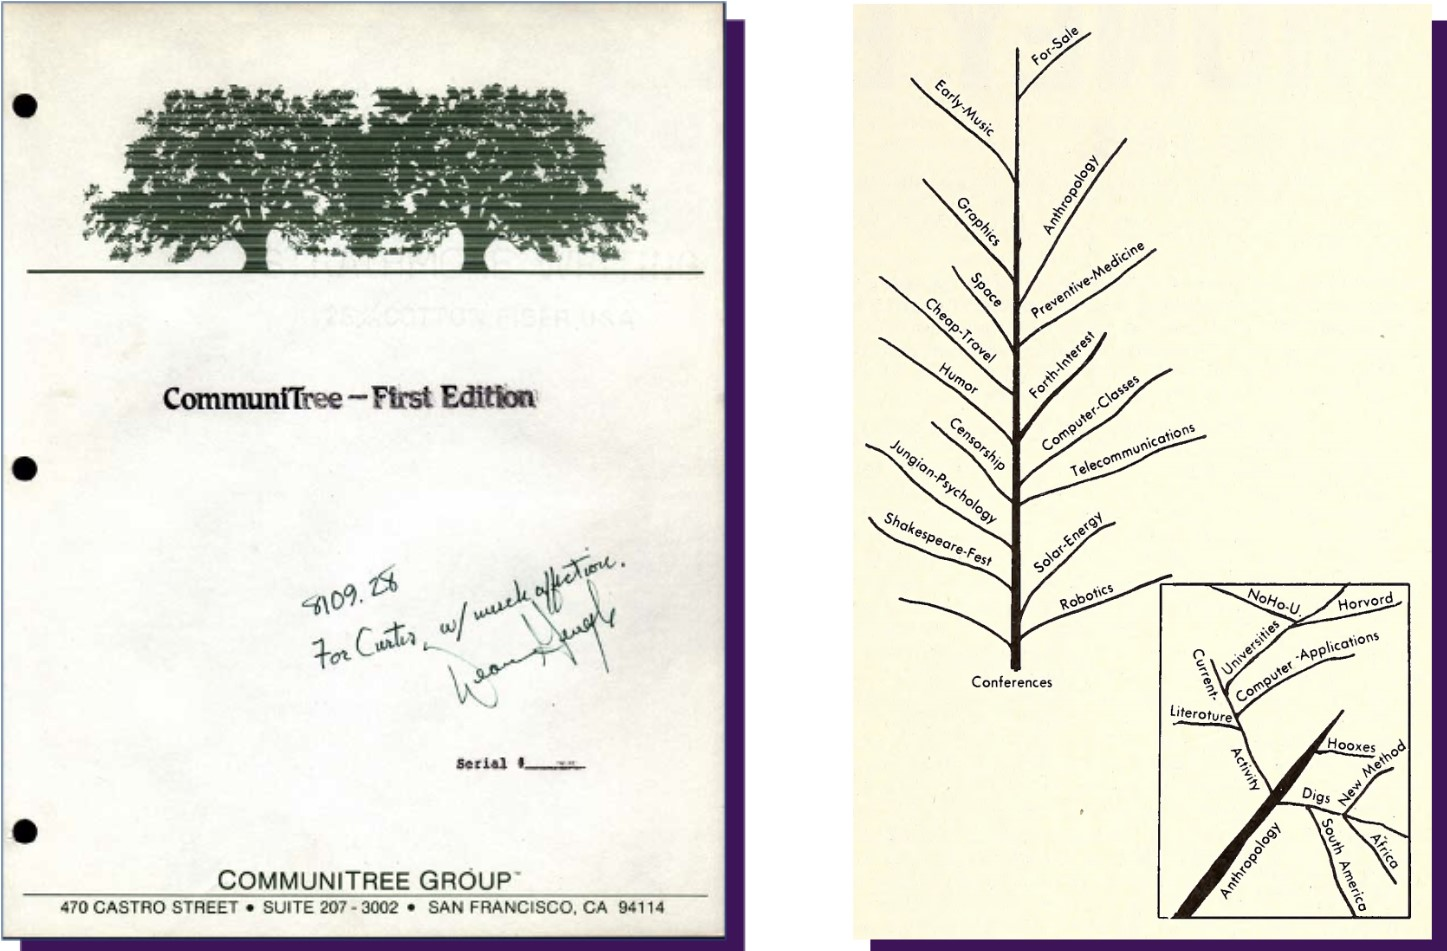
\includegraphics[width=10cm]{img/fig1.jpg}

\note[]{I want to begin with a story about the early history of content moderation. In 1978, an Electronic Bulletin Board Service called CommuniTree was founded by tech entrepreneurs in the San Francisco area as one of the first publicly accessible online communities. }
\end{frame}

%%%%%%%%%%%%%%%%%%%%%%%%%%%%%%%%%%%%%%%%%%%%%%%%
%%%%%%%%%%%%%%%%  SLIDE 4  %%%%%%%%%%%%%%%%%%%%%
%%%%%%%%%%%%%%%%%%%%%%%%%%%%%%%%%%%%%%%%%%%%%%%%
\begin{frame}{}

\vspace{0.8cm} % looks a bit more centered this way, can remove
\centering

\huge{\textbf{“We are as gods and might as well get good at it”}}

\note[]{It was built on a strong, cyber-utopian ethos inspired by figures like Stuart Brand and R. Buckminster Fuller. Its creators felt that they were at the vanguard of a digital revolution, and they weren’t shy about sharing this sense of self-importance. The very first post made to CommuniTree opened with a Stuart Brand quote – ``We are as gods and might as well get good at it''}

\end{frame}

%%%%%%%%%%%%%%%%%%%%%%%%%%%%%%%%%%%%%%%%%%%%%%%%
%%%%%%%%%%%%%%%%  SLIDE 5  %%%%%%%%%%%%%%%%%%%%%
%%%%%%%%%%%%%%%%%%%%%%%%%%%%%%%%%%%%%%%%%%%%%%%%
\begin{frame}{ANTI-CENSORSHIP ETHOS}

\vspace{10ex}

\includegraphics[scale=0.4]{img/fig2.3.jpg}
\hfill
\begin{minipage}[b]{0.5\textwidth}
    \raggedright % not sure if this does anything; tried to adjust spacing
    \small{
    \begin{itemize}
        \item System admins \hlc[brown!25]{could not filter} incoming messages
        \item \hlc[brown!25]{Difficult to remove} posted messages
        \item Anyone could use \hlc[brown!25]{``control characters''}
    \end{itemize} 
    }
\end{minipage}

\vspace{10ex}
\scriptsize{\color{lightgray}(Stone 1991, 1993)}

\note[]{Part of the underlying ethos built directly into the structure of CommuniTree was a strong aversion to anything resembling censorship. System operators couldn’t filter incoming messages to screen out problematic content, it was difficult to remove messages once they were posted, and any user could use what were called ``control characters'', basically giving them a subset of administrative powers.}
\end{frame}


%%%%%%%%%%%%%%%%%%%%%%%%%%%%%%%%%%%%%%%%%%%%%%%%
%%%%%%%%%%%%%%%%  SLIDE 6  %%%%%%%%%%%%%%%%%%%%%
%%%%%%%%%%%%%%%%%%%%%%%%%%%%%%%%%%%%%%%%%%%%%%%%
\begin{frame}{}
\vspace{10ex}
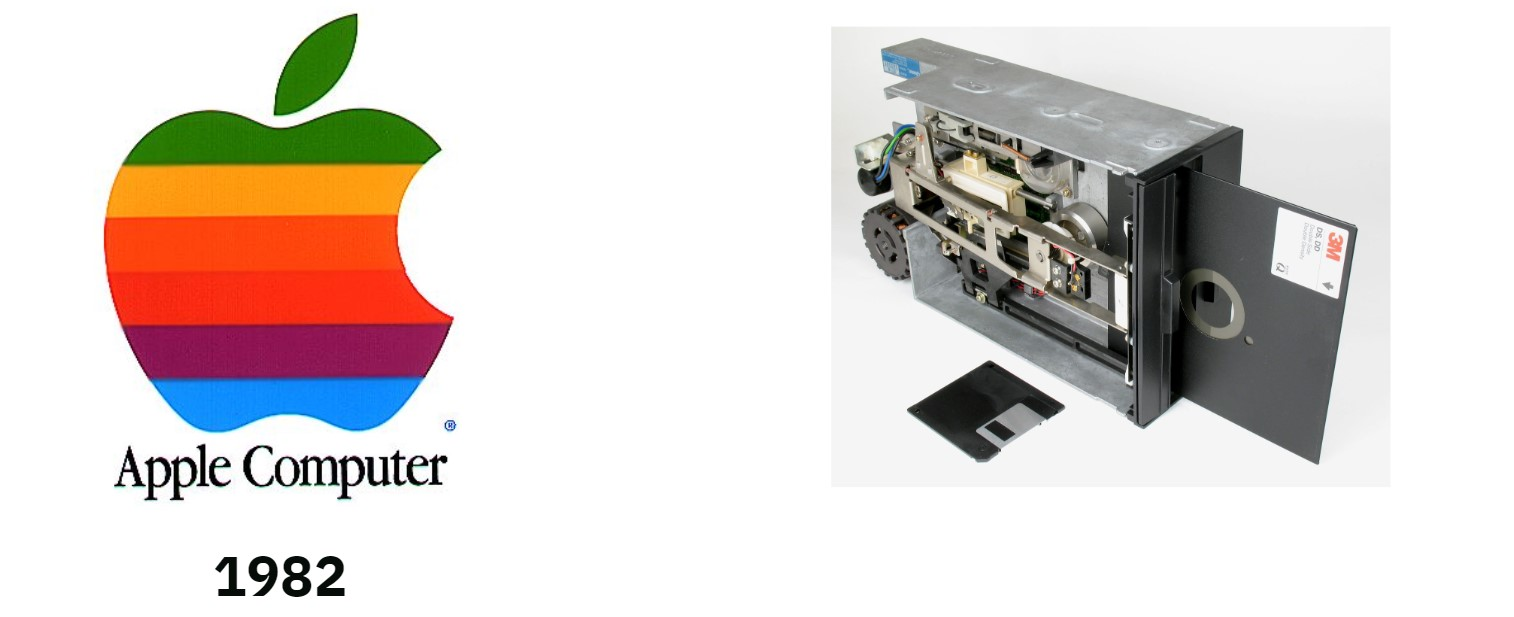
\includegraphics[scale=.325]{img/fig3.2.jpg}

\vspace{11.5ex}
\scriptsize{\color{lightgray}(Stone 1991, 1993)}

\note[]{In 1982, Apple made deal with the government to install computers into high schools in exchange for tax breaks, and enterprising high schoolers quickly discovered CommuniTree. Unimpressed by the intellectual and pseudo-spiritual attitudes of CommuniTree’s citizens, they expressed their opinions by filling the board with all manner of messages that better matched their level of maturity. Per an account from Stone, 1993 (\url{http://software.bbsdocumentary.com/APPLE/II/COMMUNITREE/vampires-excerpt.txt}): “it didn't take long for the kids to fill every byte of disk space with every word they could think of that meant shitting or fucking, and then they'd add control characters on top of that, characters that could mess with the program or stop the floppy drives. The sysops couldn't see the messages arriving and couldn't remove them afterward. The Tree was doomed.”
\newline

Within a few months, CommuniTree was dead.
}
\end{frame}


%%%%%%%%%%%%%%%%%%%%%%%%%%%%%%%%%%%%%%%%%%%%%%%%
%%%%%%%%%%%%%%%%  SLIDE 7  %%%%%%%%%%%%%%%%%%%%%
%%%%%%%%%%%%%%%%%%%%%%%%%%%%%%%%%%%%%%%%%%%%%%%%
\begin{frame}{}
\centering

\vspace{2ex}
\textbf{\huge{\emph{“We are as gods”}}}

\vspace{3ex}
\textbf{\LARGE{vs}}

\vspace{3ex}

\textbf{\huge{\emph{Teenagers }}}\pause  
\includegraphics[scale=0.06]{img/fig4.jpg}


\note[]{So – at the beginning of the social internet, gods fought teenagers, and teenagers won.}
\end{frame}


%%%%%%%%%%%%%%%%%%%%%%%%%%%%%%%%%%%%%%%%%%%%%%%%
%%%%%%%%%%%%%%%%  SLIDE 8  %%%%%%%%%%%%%%%%%%%%%
%%%%%%%%%%%%%%%%%%%%%%%%%%%%%%%%%%%%%%%%%%%%%%%%
\begin{frame}{}

\vspace{3ex}
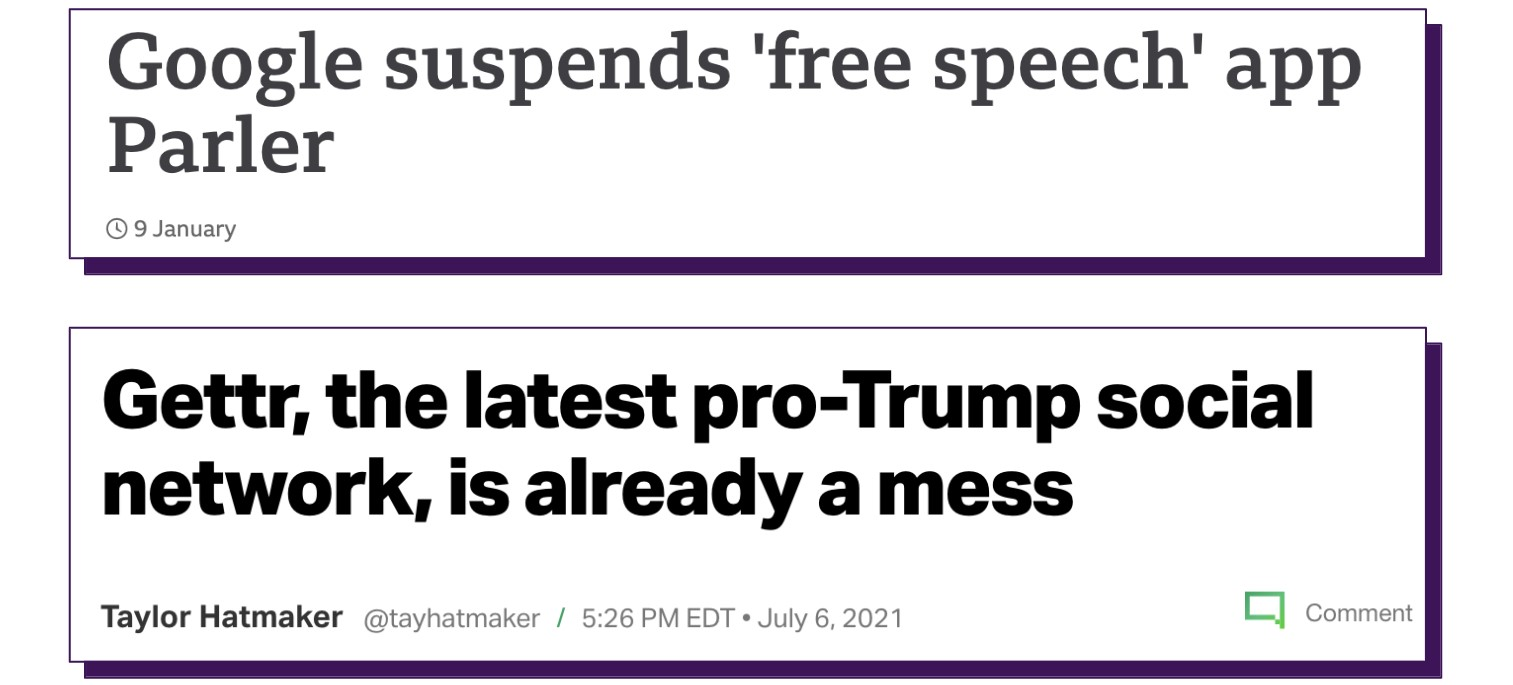
\includegraphics[width=\textwidth]{img/fig5.jpg}

\note[]{This might seem like a bit of a quaint story, but if you take a minute to think about it, it actually sounds quite a bit like something that could still happen today, more than 40 years later. Despite clear evidence from over decades, new platforms and spaces are still created with this same sort of free speech, anti-censorship ethos and are woefully underprepared when things don’t go as planned. }
\end{frame}


%%%%%%%%%%%%%%%%%%%%%%%%%%%%%%%%%%%%%%%%%%%%%%%%
%%%%%%%%%%%%%%%%  SLIDE 9  %%%%%%%%%%%%%%%%%%%%%
%%%%%%%%%%%%%%%%%%%%%%%%%%%%%%%%%%%%%%%%%%%%%%%%
\begin{frame}{}

\vspace{2ex}
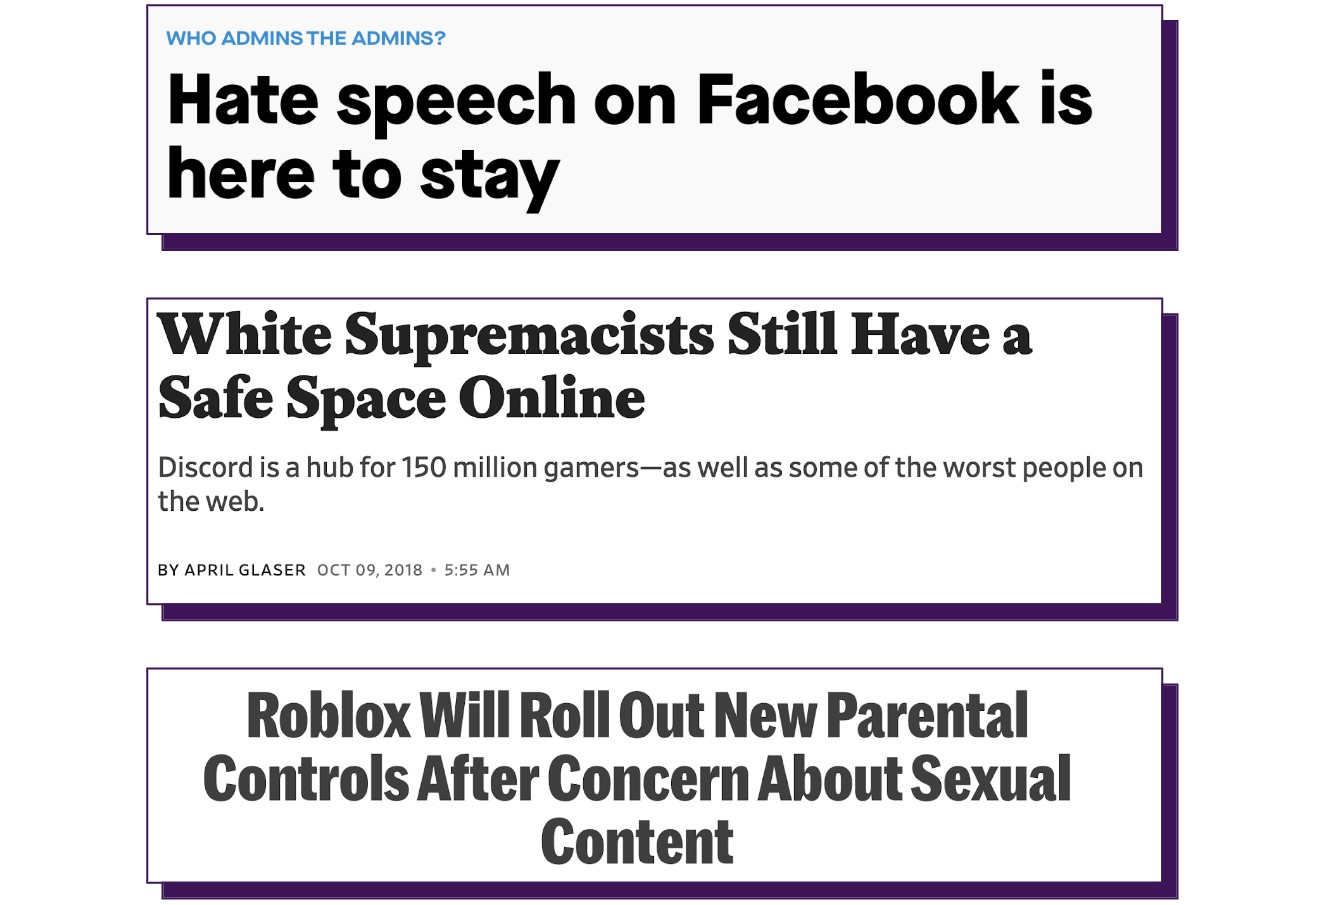
\includegraphics[width=\textwidth]{img/fig6.jpg}

\note[]{And the issues at play can be far more complex and dangerous than teenagers making crude posts – as we’ve seen throughout the other modules, content moderation has really become a core part of ensuring a functioning society.}
\end{frame}


%%%%%%%%%%%%%%%%%%%%%%%%%%%%%%%%%%%%%%%%%%%%%%%%
%%%%%%%%%%%%%%%%  SLIDE 10  %%%%%%%%%%%%%%%%%%%%%
%%%%%%%%%%%%%%%%%%%%%%%%%%%%%%%%%%%%%%%%%%%%%%%%
\begin{frame}{How Do We Talk About Moderation}


\includegraphics[width=\textwidth]{img/fig7.1.jpg}

\note[]{When we talk about content moderation, we often hear language that invokes metaphors of government and regulation – two of the seminal publications describing the current era of content moderation are titled “The New Governors” and “Digital Constitutionalism”. In this module though, I’m going to encourage you to think a little more broadly about how you view content moderation.}
\end{frame}


%%%%%%%%%%%%%%%%%%%%%%%%%%%%%%%%%%%%%%%%%%%%%%%%
%%%%%%%%%%%%%%%%  SLIDE 11  %%%%%%%%%%%%%%%%%%%%%
%%%%%%%%%%%%%%%%%%%%%%%%%%%%%%%%%%%%%%%%%%%%%%%%
\begin{frame}{Consequences of Regulatory Framing?}

\vspace{-9ex} % trying to get the spacing right both vertically and horizontally
\hspace{1ex}
\begin{minipage}[c][1ex][t]{0.4\textwidth}
    
\includegraphics[scale=0.4]{img/fig8.jpg}
\end{minipage}

\hspace{25ex}
\begin{minipage}[c][2ex][c]{0.5\textwidth}
    \begin{itemize}
        \item Universal policies
        \item Reactive punishments
    \end{itemize} 
\end{minipage}

\note[]{Thinking about content moderation as a regulatory process traps us in a reactive mindset: we write rules, and when those rules are broken, we administer punishments.}
\end{frame}


%%%%%%%%%%%%%%%%%%%%%%%%%%%%%%%%%%%%%%%%%%%%%%%%
%%%%%%%%%%%%%%%%  SLIDE 12  %%%%%%%%%%%%%%%%%%%%%
%%%%%%%%%%%%%%%%%%%%%%%%%%%%%%%%%%%%%%%%%%%%%%%%
\begin{frame}{}

\centering
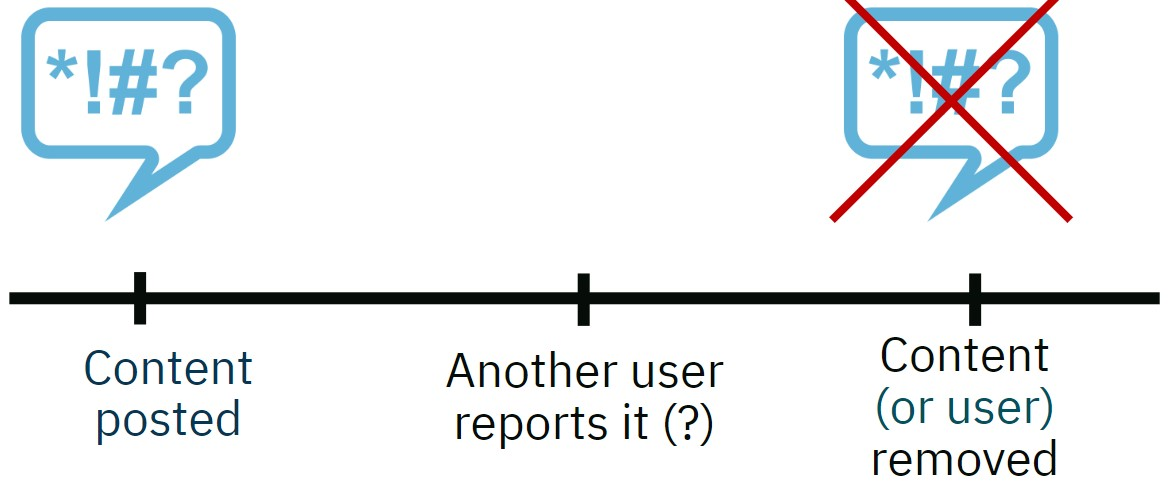
\includegraphics[width=\textwidth]{img/fig9.jpg}

\note[]{This sort of mindset might imagine the content moderation process as taking place during the period of time between when a piece of content is posted and when action is (or isn’t) taken on it, sometimes with user reports in between.}
\end{frame}


%%%%%%%%%%%%%%%%%%%%%%%%%%%%%%%%%%%%%%%%%%%%%%%%
%%%%%%%%%%%%%%%%  SLIDE 13  %%%%%%%%%%%%%%%%%%%%%
%%%%%%%%%%%%%%%%%%%%%%%%%%%%%%%%%%%%%%%%%%%%%%%%
\begin{frame}{}

\vspace*{5ex}
\centering
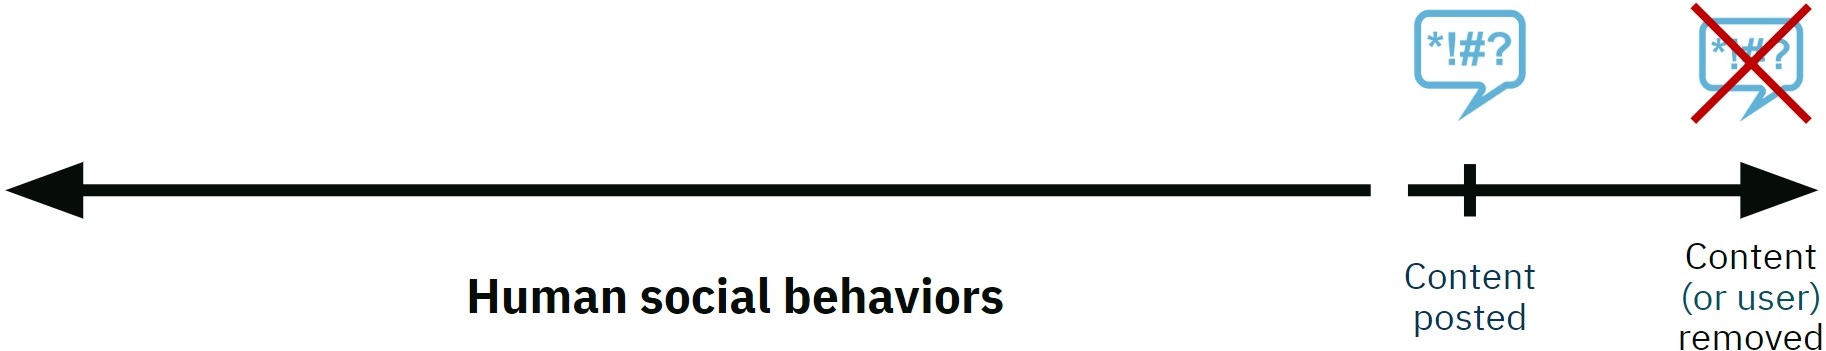
\includegraphics[width=\textwidth]{img/fig10.jpg} 

\note[]{However, it can be much more productive to zoom out and consider both the period of time leading up to when content is posted and the period of time after action is taken. In the lead-up period, we can often see signs that something may not be going quite right, and in the aftermath we can see the impact of actions taken on affected users, onlookers, and even more broadly.}

\end{frame}

%%%%%%%%%%%%%%%%%%%%%%%%%%%%%%%%%%%%%%%%%%%%%%%%
%%%%%%%%%%%%%%%%  SLIDE 14  %%%%%%%%%%%%%%%%%%%%%
%%%%%%%%%%%%%%%%%%%%%%%%%%%%%%%%%%%%%%%%%%%%%%%%
\begin{frame}{Models for content moderation?}

\vspace*{3ex}
\large{
\begin{enumerate}
    \item Artisanal
    \item Community-reliant
    \item Industrial
\end{enumerate}
}

\vspace{22ex}
\scriptsize{\color{lightgray}Caplan, 2018}

\note[]{Researchers often use a framework developed by Robyn Caplan to categorize different approaches to content moderation. She identifies three approaches: \newline

Artisanal – where decisions are made in-house at companies on a case-by-case basis \newline

Community-reliant – where decisions are made by networks or committees of volunteer users \newline

Industrial – where decisions are made by specialized enforcement teams, often with the assistance of automation and hired contractors, usually separate from policy teams
}
\end{frame}


%%%%%%%%%%%%%%%%%%%%%%%%%%%%%%%%%%%%%%%%%%%%%%%%
%%%%%%%%%%%%%%%%  SLIDE 15  %%%%%%%%%%%%%%%%%%%%%
%%%%%%%%%%%%%%%%%%%%%%%%%%%%%%%%%%%%%%%%%%%%%%%%
\begin{frame}{}

\vspace*{5ex}
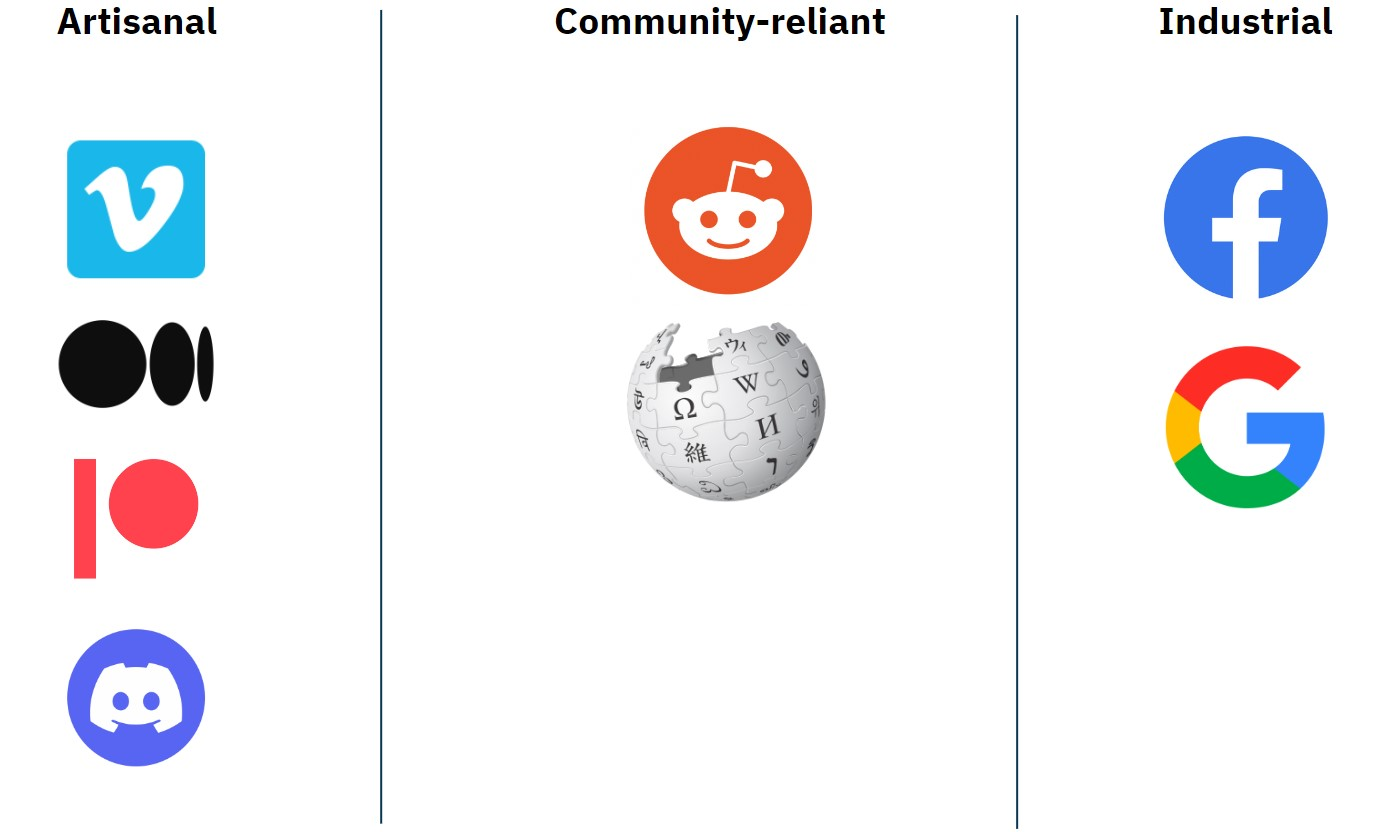
\includegraphics[width=\textwidth]{img/fig11.jpg}

\vfill
\vspace{5ex}
\scriptsize{\color{lightgray}Caplan, 2018}

\note[]{In her 2018 paper where she defined these categories, Caplan gave a number of examples of platforms that fell into each – she listed Vimeo, Medium, Patreon, and Discord as Artisanal companies; Reddit and Wikimedia as Community-reliant; and Facebook and Google as Industrial.}

\end{frame}

%%%%%%%%%%%%%%%%%%%%%%%%%%%%%%%%%%%%%%%%%%%%%%%%
%%%%%%%%%%%%%%%%  SLIDE 16  %%%%%%%%%%%%%%%%%%%%%
%%%%%%%%%%%%%%%%%%%%%%%%%%%%%%%%%%%%%%%%%%%%%%%%
\begin{frame}{}

\vspace*{6ex}

\huge{\textbf{But...}}

\note[]{There are really elements of each in all of these.}

\end{frame}


%%%%%%%%%%%%%%%%%%%%%%%%%%%%%%%%%%%%%%%%%%%%%%%%
%%%%%%%%%%%%%%%%  SLIDE 17  %%%%%%%%%%%%%%%%%%%%%
%%%%%%%%%%%%%%%%%%%%%%%%%%%%%%%%%%%%%%%%%%%%%%%%
\begin{frame}{}


\includegraphics[width = \textwidth]{img/fig12.jpg}

\note[]{As I was working on these slides I tried my best to think about all the platforms I could remember that are moderated in some nontrivial part by volunteers, and these are the ones I came up with kind of off the top of my head. Most academic research has focused on a subset of these (circled), but volunteer moderation is actually sneakily part of a lot of different ecosystems that people don’t often think about. For example…}
\end{frame}


%%%%%%%%%%%%%%%%%%%%%%%%%%%%%%%%%%%%%%%%%%%%%%%%
%%%%%%%%%%%%%%%%  SLIDE 18  %%%%%%%%%%%%%%%%%%%%%
%%%%%%%%%%%%%%%%%%%%%%%%%%%%%%%%%%%%%%%%%%%%%%%%
\begin{frame}{}

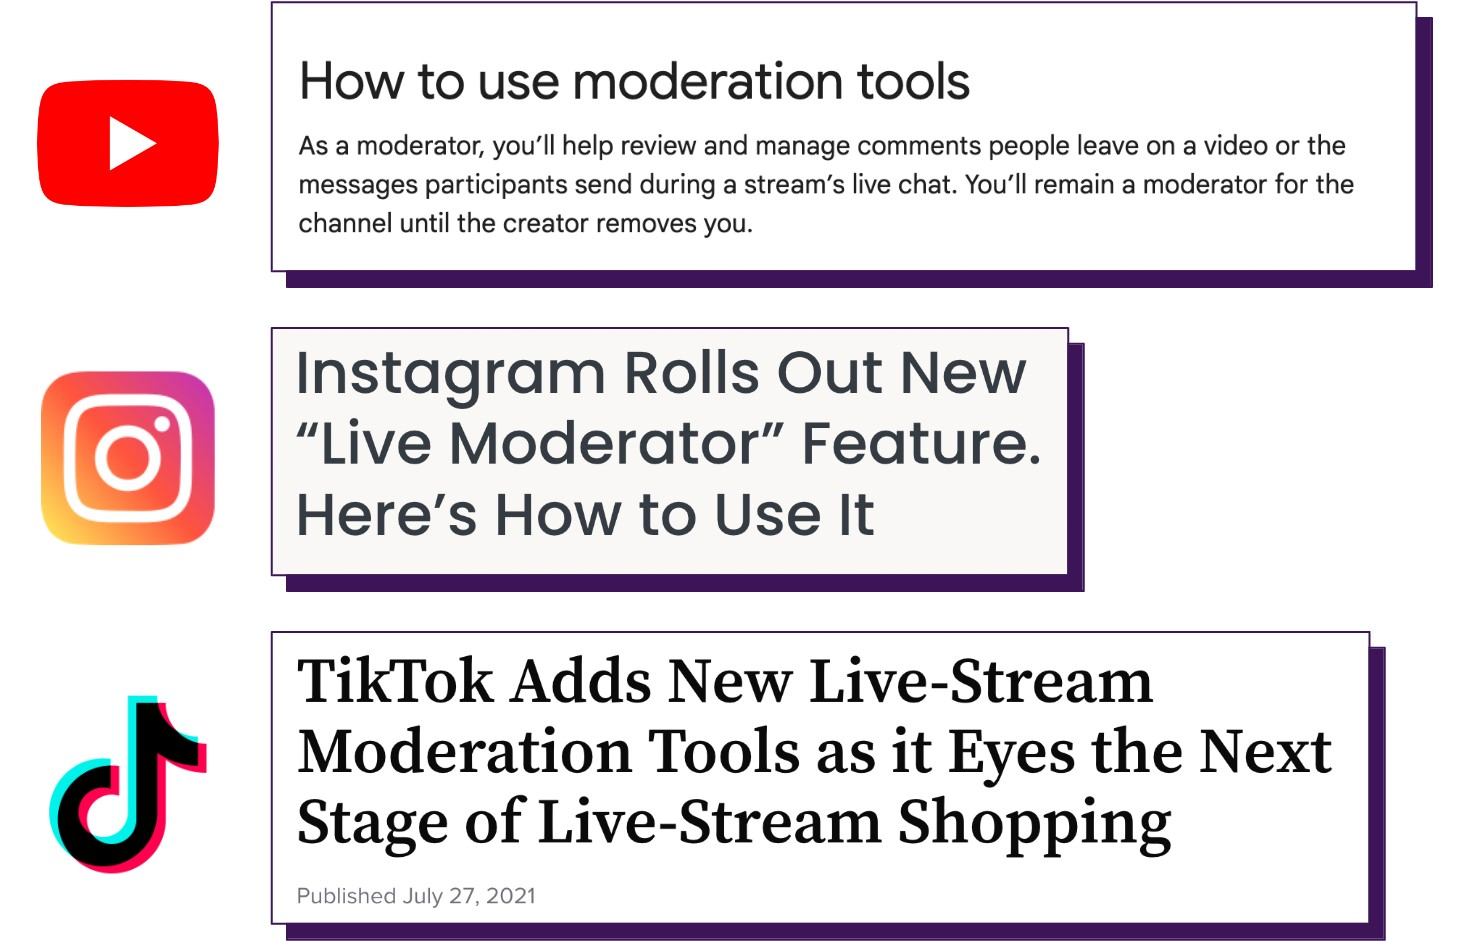
\includegraphics[width=\textwidth]{img/fig13.jpg}

\note[]{Beyond the platforms that we usually think about as being moderated by volunteers, designated volunteers can actually moderate comments and users on things like tiktok and youtube and instagram livestreams, and instagram and youtube creators can moderate comments on their posts at least to a certain extent. It’s a little hard to find out about these tools and functions because the documentation is pretty thin, but it’s definitely something that does happen.
}
\end{frame}


%%%%%%%%%%%%%%%%%%%%%%%%%%%%%%%%%%%%%%%%%%%%%%%%
%%%%%%%%%%%%%%%%  SLIDE 19  %%%%%%%%%%%%%%%%%%%%%
%%%%%%%%%%%%%%%%%%%%%%%%%%%%%%%%%%%%%%%%%%%%%%%%
\begin{frame}{What’s the scale?}

\small{
\textbf{\hlc[brown!30]{70+ million}} Facebook group/page moderators as of 2020
\newline \newline
Much of Reddit has been moderated by volunteers since 2005
\newline \newline
On Discord, volunteers moderate servers that have up to \textbf{\hlc[brown!30]{many  hundreds  of  thousands}} of users
}

\note[]{So what’s the scale of this? Beyond just how many platforms rely on volunteer moderators, they actually do quite a lot of work. Facebook is of course the behemoth in this space, and I wish we had more updated numbers on this, but as of 2020 there were more than 70 million volunteers moderating groups and pages, and even if only one percent of those are active at all, that’s still quite a lot of moderators. \newline

(\url{https://www.facebook.com/community/whats-new/facebook-communities-summit-keynote-recap/}
}
\end{frame}


%%%%%%%%%%%%%%%%%%%%%%%%%%%%%%%%%%%%%%%%%%%%%%%%
%%%%%%%%%%%%%%%%  SLIDE 20  %%%%%%%%%%%%%%%%%%%%%
%%%%%%%%%%%%%%%%%%%%%%%%%%%%%%%%%%%%%%%%%%%%%%%%
\begin{frame}{What this looks like on Twitch}

\vspace*{7ex}
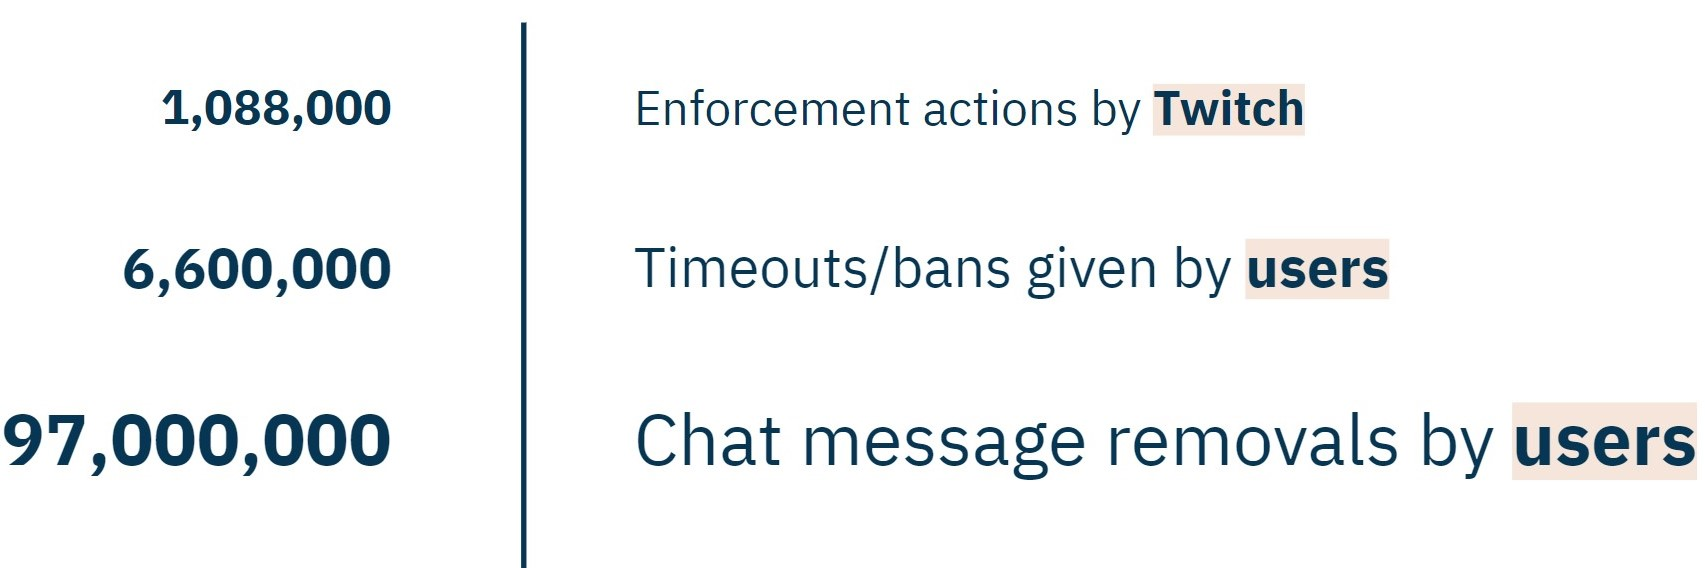
\includegraphics[width = \textwidth]{img/fig14.1.jpg}
\vfill
\vspace{12ex}
\scriptsize{\color{lightgray}(H1 2022)}

\note[]{To give you another perspective on scale, here are some numbers from Twitch’s transparency report, I think this was the first half of 2022. \newline 
(\url{https://safety.twitch.tv/s/article/H1-2022-Transparency-Report?language=en_US}) \newline

About 20\% of those 97,000,000 were manual removals, and the rest were removed by automated tools based on settings the users manage. \newline 

Apologies to current and former Twitch folks here, this isn’t a totally fair comparison, but it should give a sense of the scale of how big this is.
}
\end{frame}


%%%%%%%%%%%%%%%%%%%%%%%%%%%%%%%%%%%%%%%%%%%%%%%%
%%%%%%%%%%%%%%%%  SLIDE 21 part 1  %%%%%%%%%%%%%%%%%%%%%
%%%%%%%%%%%%%%%%%%%%%%%%%%%%%%%%%%%%%%%%%%%%%%%%
\begin{frame}{But More Broadly?}

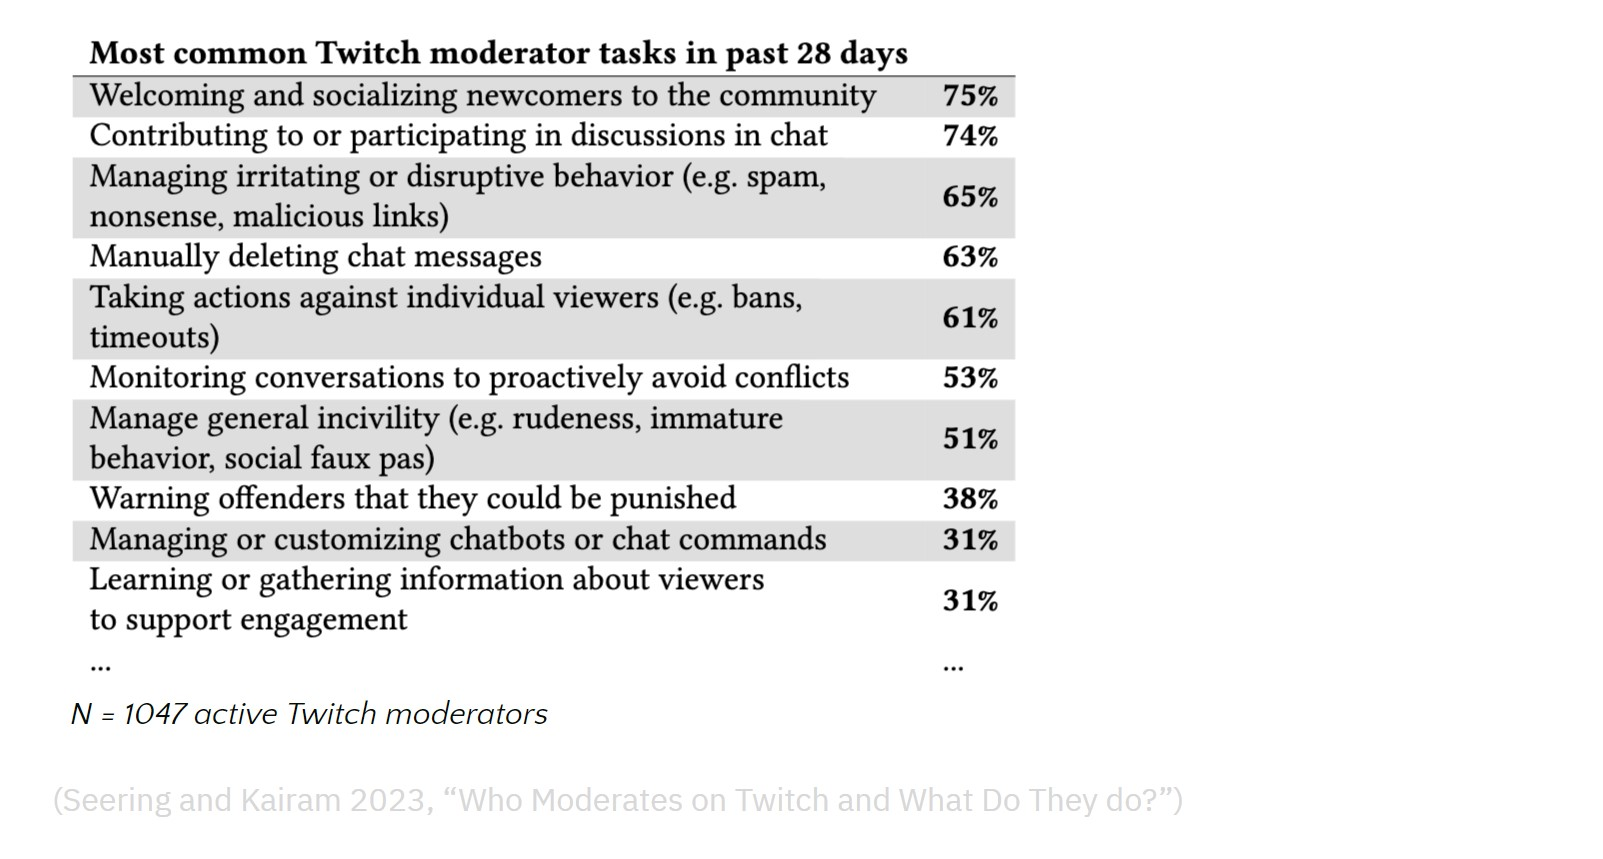
\includegraphics[width=\textwidth]{img/fig15.jpg}

\note[]{Now to be fair, moderators do a lot more than just removing stuff. This is from some recently published work that I did with Sanjay actually about what volunteer moderators do on Twitch, and they definitely do some of this removal and banning work, but a lot of what they do is much more social.}

\end{frame}


%%%%%%%%%%%%%%%%%%%%%%%%%%%%%%%%%%%%%%%%%%%%%%%%
%%%%%%%%%%%%%%%%  SLIDE 21 part 2  %%%%%%%%%%%%%%%%%%%%%
%%%%%%%%%%%%%%%%%%%%%%%%%%%%%%%%%%%%%%%%%%%%%%%%
\begin{frame}{But More Broadly?}

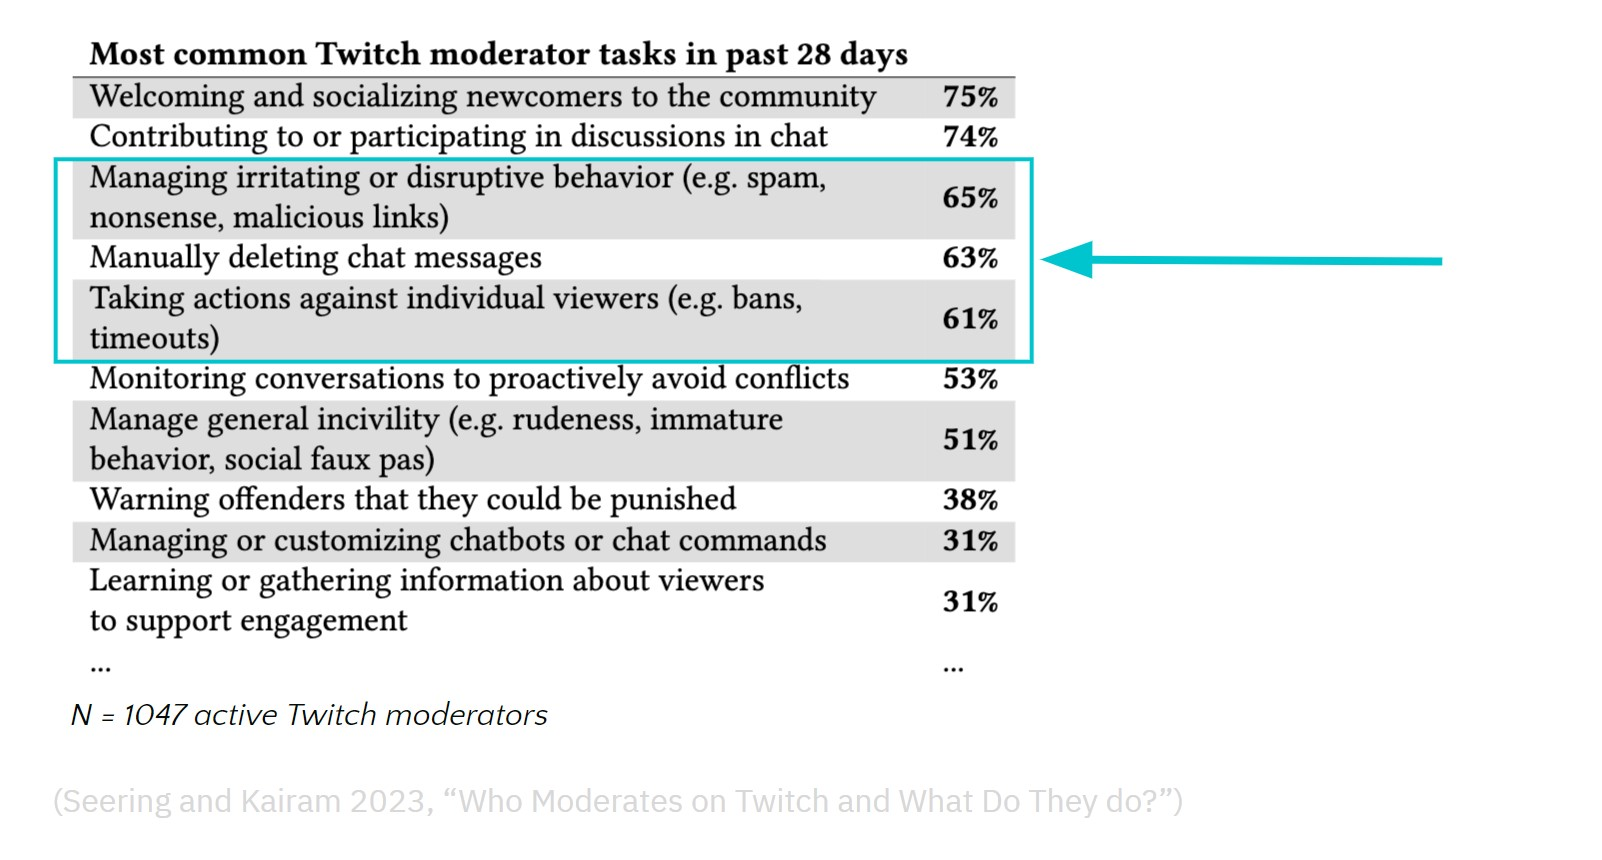
\includegraphics[width=\textwidth]{img/fig15.1.jpg}

\note[]{Now to be fair, moderators do a lot more than just removing stuff. This is from some recently published work that I did with Sanjay actually about what volunteer moderators do on Twitch, and they definitely do some of this removal and banning work, but a lot of what they do is much more social.}

\end{frame}




%%%%%%%%%%%%%%%%%%%%%%%%%%%%%%%%%%%%%%%%%%%%%%%%
%%%%%%%%%%%%%%%%  SLIDE 21 part 3 %%%%%%%%%%%%%%%%%%%%%
%%%%%%%%%%%%%%%%%%%%%%%%%%%%%%%%%%%%%%%%%%%%%%%%
\begin{frame}{But More Broadly?}

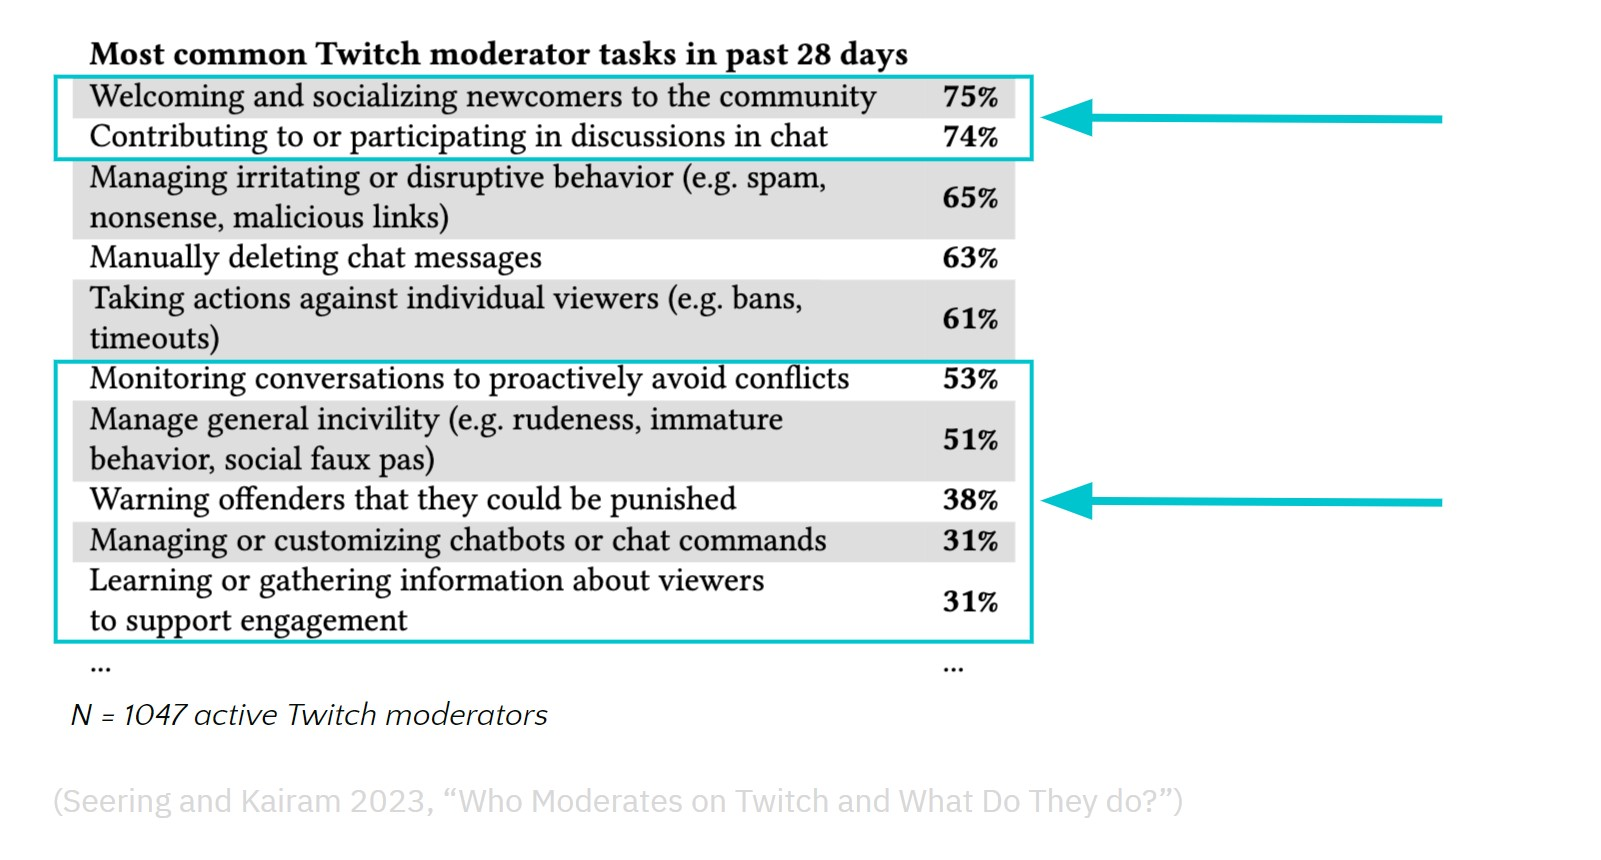
\includegraphics[width=\textwidth]{img/fig15.2.jpg}

\note[]{Now to be fair, moderators do a lot more than just removing stuff. This is from some recently published work that I did with Sanjay actually about what volunteer moderators do on Twitch, and they definitely do some of this removal and banning work, but a lot of what they do is much more social.}

\end{frame}


%%%%%%%%%%%%%%%%%%%%%%%%%%%%%%%%%%%%%%%%%%%%%%%%
%%%%%%%%%%%%%%%%  SLIDE 22  %%%%%%%%%%%%%%%%%%%%%
%%%%%%%%%%%%%%%%%%%%%%%%%%%%%%%%%%%%%%%%%%%%%%%%
%\begin{frame}{Looking at communities}

%Why should we look at small, user-run spaces?

%\note[]{
%Well, 
%}

%\end{frame}


%%%%%%%%%%%%%%%%%%%%%%%%%%%%%%%%%%%%%%%%%%%%%%%%
%%%%%%%%%%%%%%%%  SLIDE 23  %%%%%%%%%%%%%%%%%%%%%
%%%%%%%%%%%%%%%%%%%%%%%%%%%%%%%%%%%%%%%%%%%%%%%%
%\begin{frame}{This slide should be about commercial content moderators}

%\end{frame}



%%%%%%%%%%%%%%%%%%%%%%%%%%%%%%%%%%%%%%%%%%%%%%%%
%%%%%%%%%%%%%%%%  SLIDE 24  %%%%%%%%%%%%%%%%%%%%%
%%%%%%%%%%%%%%%%%%%%%%%%%%%%%%%%%%%%%%%%%%%%%%%%
\begin{frame}{Breakout task one}

\normalsize{
Imagine you’re starting a wiki for your favorite game/book/ sports team/tv series.

With your group, take 5-7 minutes and write a draft set of rules that you want people to follow when contributing /commenting on your Wiki. 
}
\end{frame}

%%%%%%%%%%%%%%%%%%%%%%%%%%%%%%%%%%%%%%%%%%%%%%%%
%%%%%%%%%%%%%%%%  SLIDE 25  %%%%%%%%%%%%%%%%%%%%%
%%%%%%%%%%%%%%%%%%%%%%%%%%%%%%%%%%%%%%%%%%%%%%%%
\begin{frame}{}

\vspace*{7ex}
\begin{center}
    \LARGE{
        Part 1: Moderation \hlc[brown!30]{Processes} 
        \newline 
        \textcolor{white}{..........} and %% workaround for centering
        \newline 
        Moderators’ \hlc[brown!30]{Roles}
    }  
\end{center}

\vfill
\vspace{20ex}
\scriptsize{\color{lightgray}(Seering et al. 2019, “Moderator Engagement”; \newline 
Seering et al. 2020, “Metaphors for Moderation”)}

\end{frame}



%%%%%%%%%%%%%%%%%%%%%%%%%%%%%%%%%%%%%%%%%%%%%%%%
%%%%%%%%%%%%%%%%  SLIDE 26  %%%%%%%%%%%%%%%%%%%%%
%%%%%%%%%%%%%%%%%%%%%%%%%%%%%%%%%%%%%%%%%%%%%%%%
\begin{frame}{}

\vspace*{5ex}

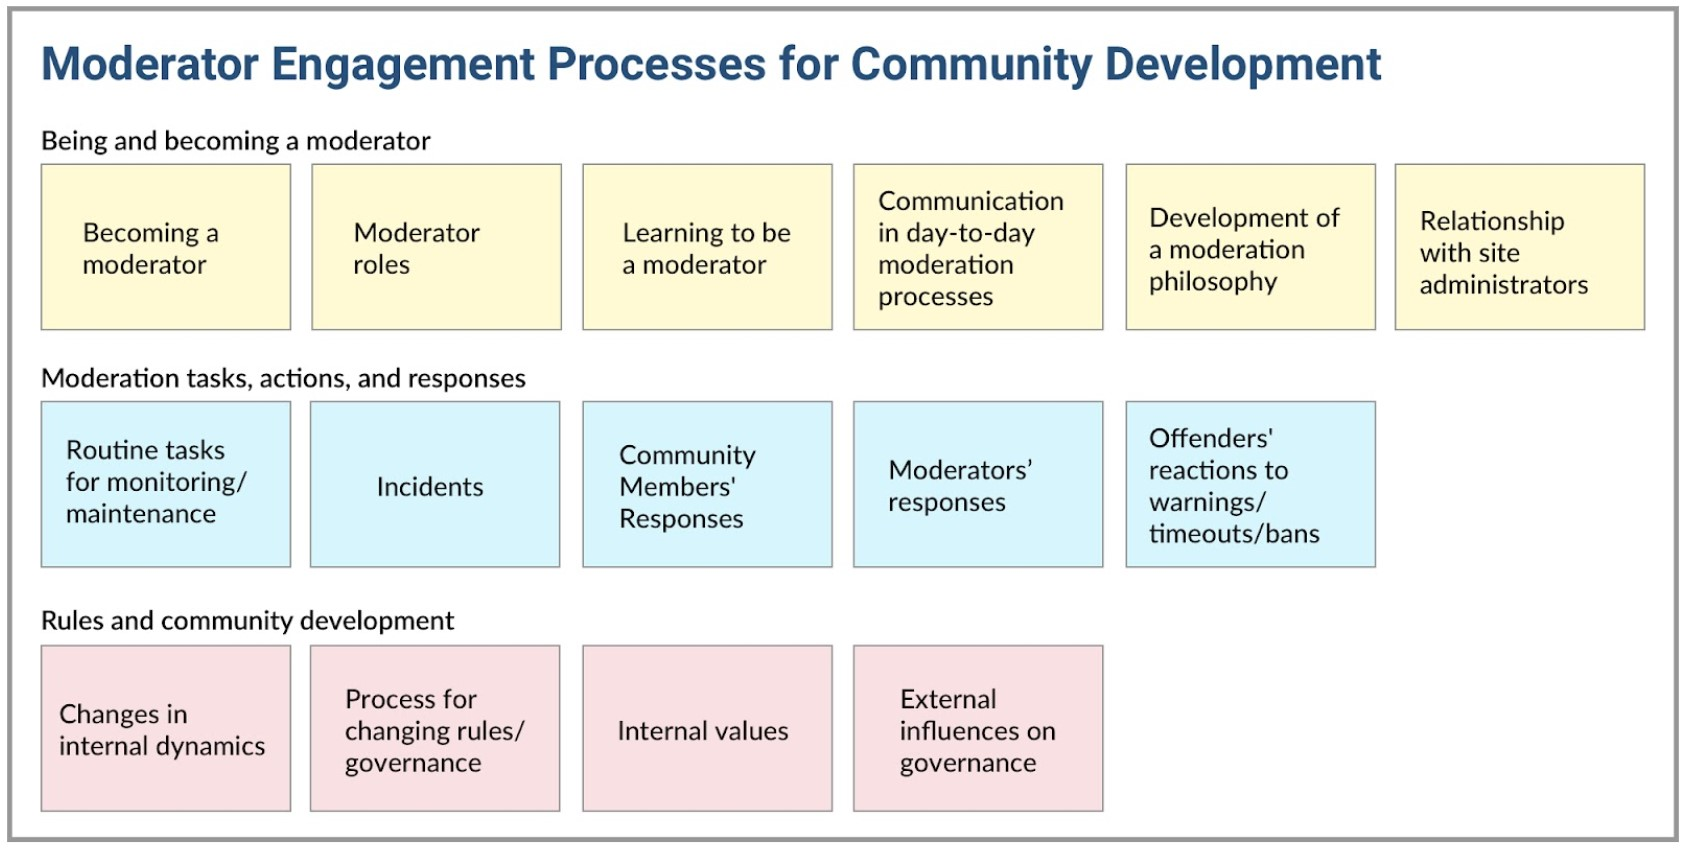
\includegraphics[width=\textwidth]{img/fig16.jpg}

\vfill
\vspace{10ex}
\scriptsize{\color{lightgray}(Seering et al. 2019, “Moderator Engagement”)}

\end{frame}

%%%%%%%%%%%%%%%%%%%%%%%%%%%%%%%%%%%%%%%%%%%%%%%%
%%%%%%%%%%%%%%%% SLIDE 27 PART 1 %%%%%%%%%%%%%%%
%%%%%%%%%%%%%%%%%%%%%%%%%%%%%%%%%%%%%%%%%%%%%%%%
\begin{frame}{}

\vspace*{1ex}
\begin{center}
   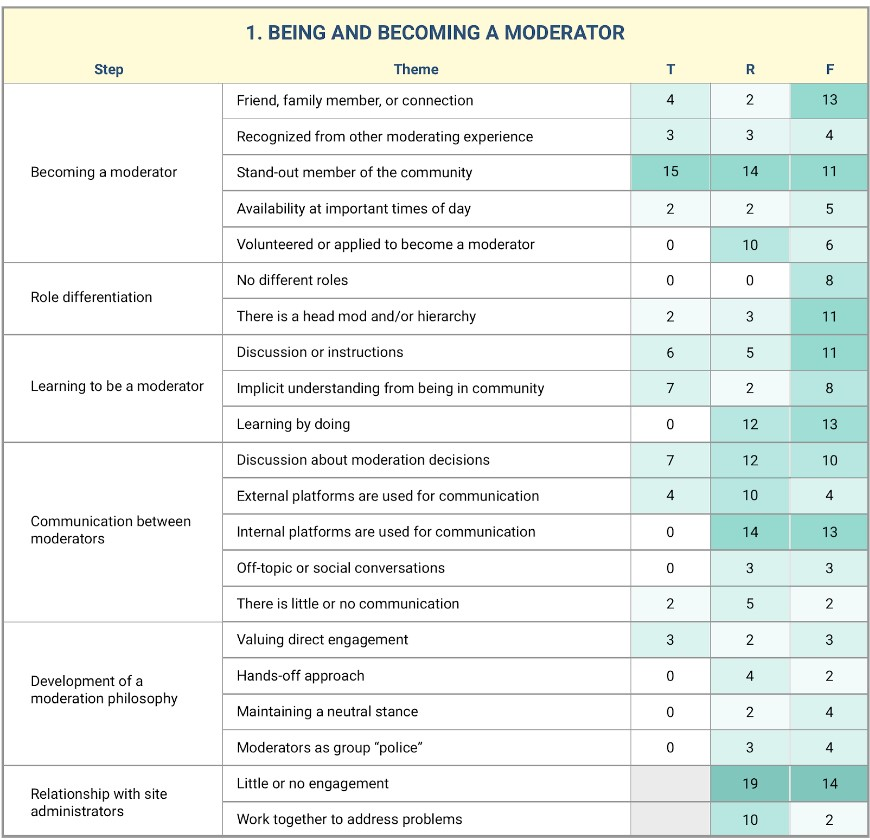
\includegraphics[scale=.425]{img/fig17.1.jpg} 
\end{center}

\vspace{5ex}
\scriptsize{\color{lightgray}(Seering et al. 2019, “Moderator Engagement”)}

\end{frame}

%%%%%%%%%%%%%%%%%%%%%%%%%%%%%%%%%%%%%%%%%%%%%%%%
%%%%%%%%%%%%%%%% SLIDE 27  PART 2 %%%%%%%%%%%%%%
%%%%%%%%%%%%%%%%%%%%%%%%%%%%%%%%%%%%%%%%%%%%%%%%
\begin{frame}{}

\begin{center}
   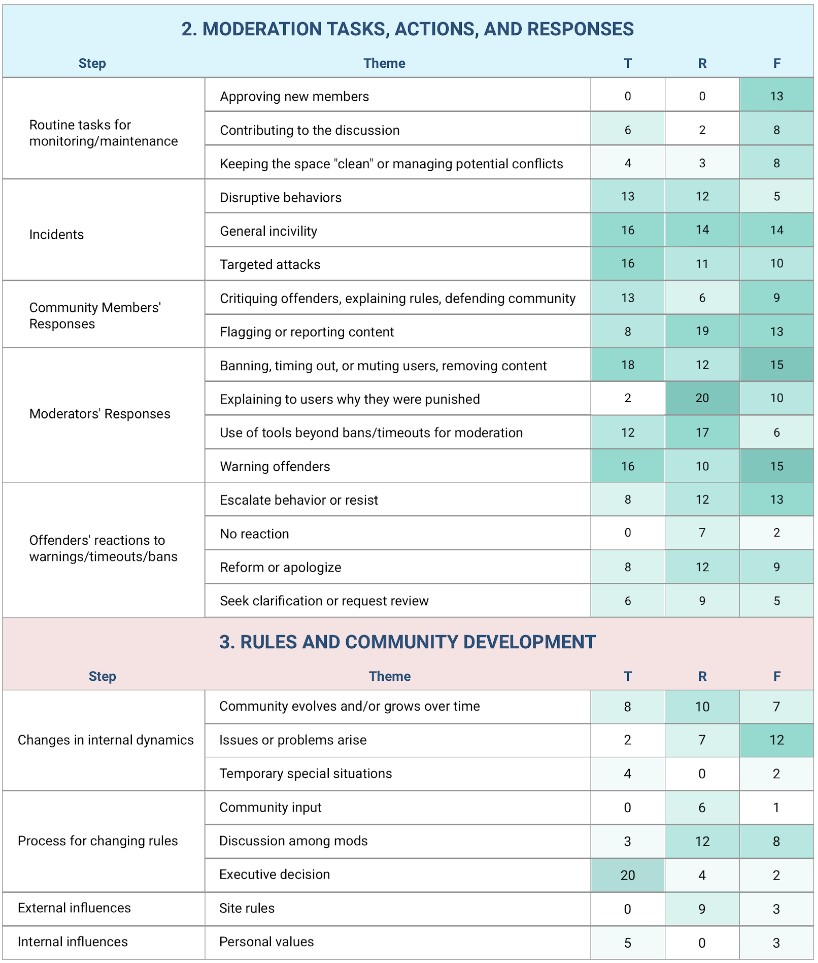
\includegraphics[scale=.425]{img/fig17.2.jpg} 
\end{center}

\scriptsize{\color{lightgray}(Seering et al. 2019, “Moderator Engagement”)}

\end{frame}



%%%%%%%%%%%%%%%%%%%%%%%%%%%%%%%%%%%%%%%%%%%%%%%%
%%%%%%%%%%%%%%%%  SLIDE 28  %%%%%%%%%%%%%%%%%%%%%
%%%%%%%%%%%%%%%%%%%%%%%%%%%%%%%%%%%%%%%%%%%%%%%%
\begin{frame}{}

\vspace*{4.5ex}

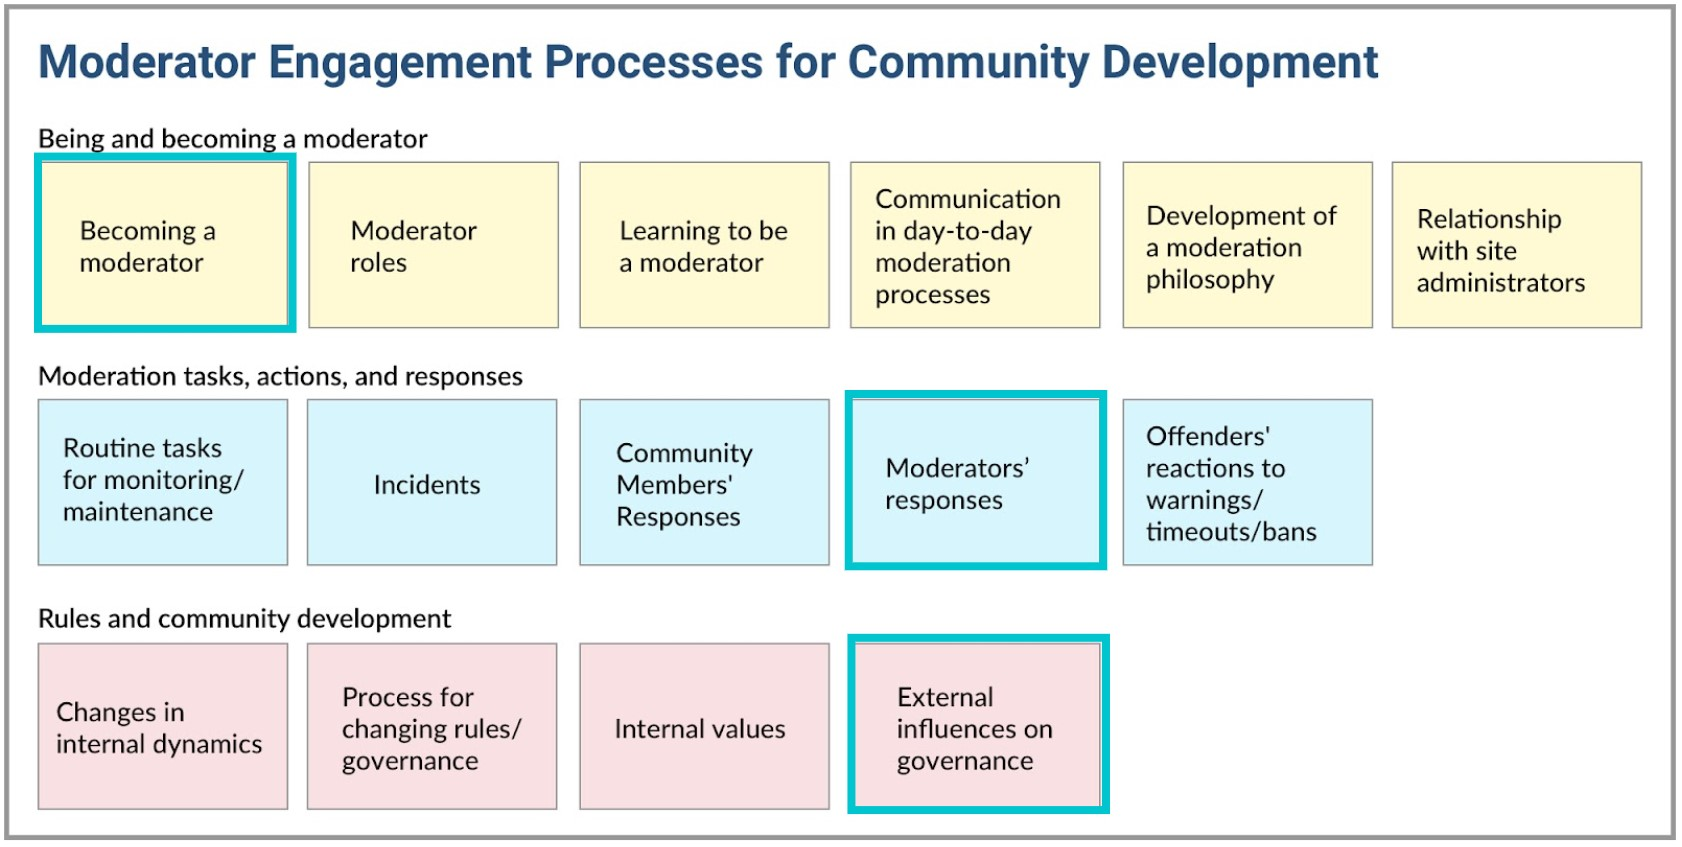
\includegraphics[width=\textwidth]{img/fig18.jpg}

\vspace{12ex}
\scriptsize{\color{lightgray}(Seering et al. 2019, “Moderator Engagement”)}

\end{frame}



%%%%%%%%%%%%%%%%%%%%%%%%%%%%%%%%%%%%%%%%%%%%%%%%
%%%%%%%%%%%%%%%%  SLIDE 29  %%%%%%%%%%%%%%%%%%%%%
%%%%%%%%%%%%%%%%%%%%%%%%%%%%%%%%%%%%%%%%%%%%%%%%
\begin{frame}{Becoming a Moderator}

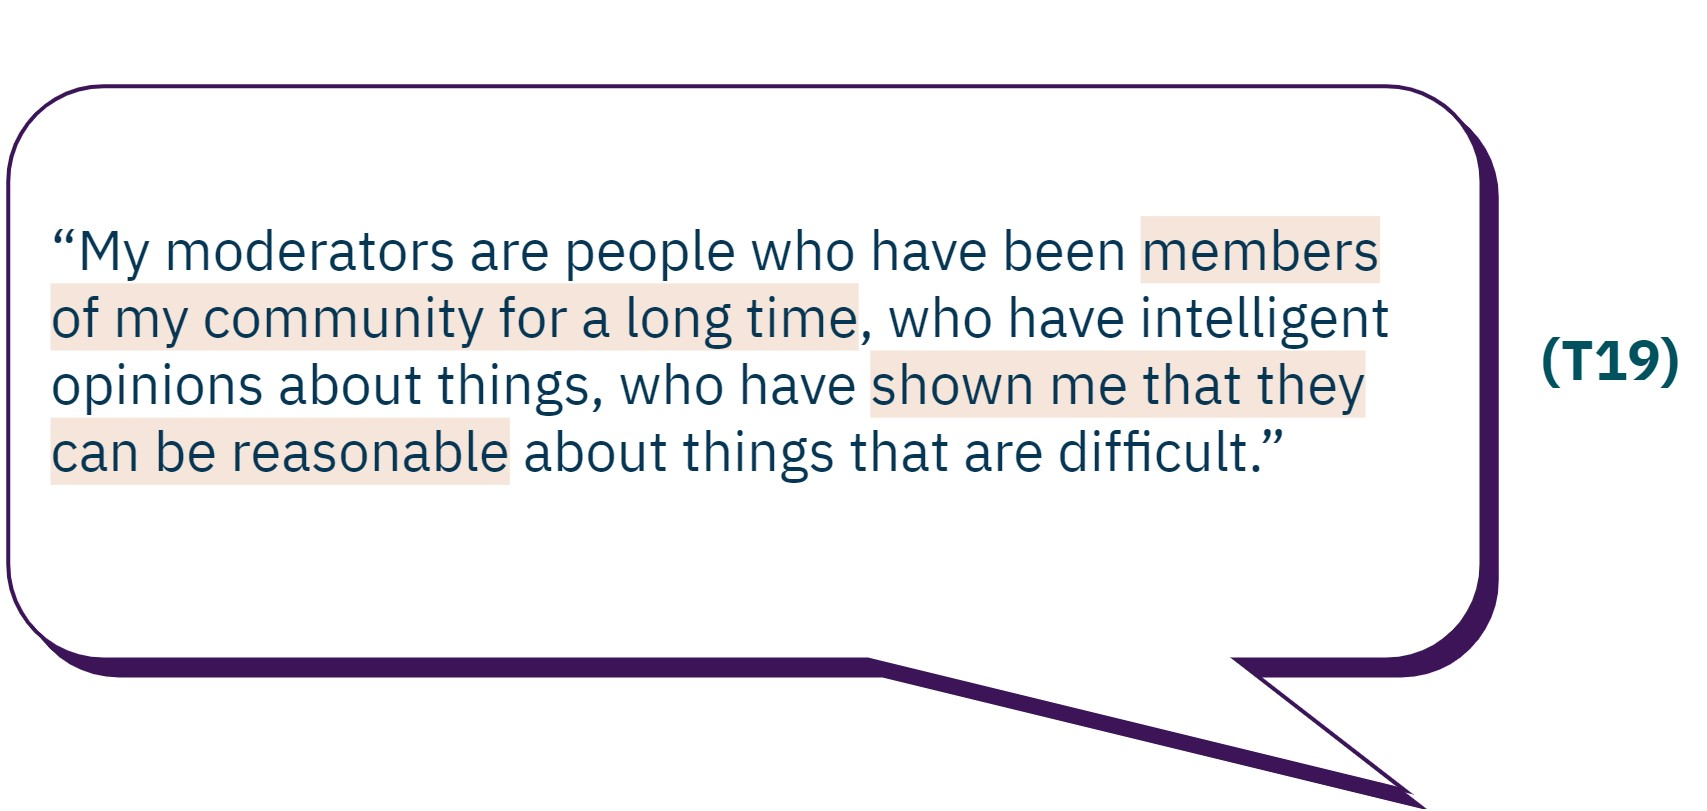
\includegraphics[width=\textwidth]{img/fig19.jpg}

\end{frame}



%%%%%%%%%%%%%%%%%%%%%%%%%%%%%%%%%%%%%%%%%%%%%%%%
%%%%%%%%%%%%%%%%  SLIDE 30  %%%%%%%%%%%%%%%%%%%%%
%%%%%%%%%%%%%%%%%%%%%%%%%%%%%%%%%%%%%%%%%%%%%%%%
\begin{frame}{}

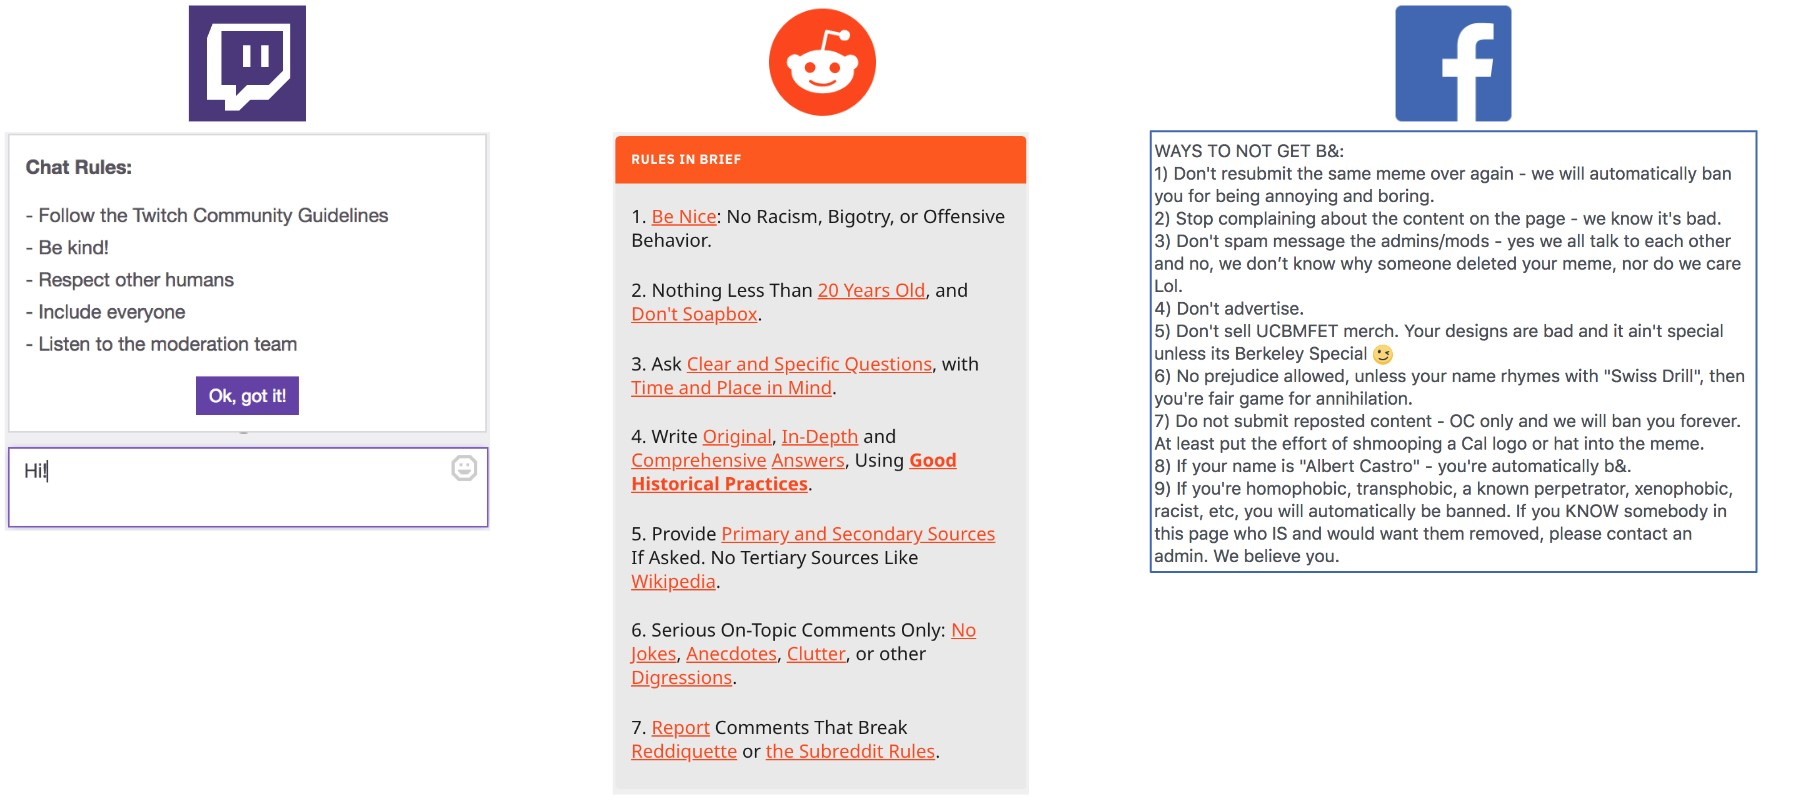
\includegraphics[width=\textwidth]{img/fig20.jpg}

\end{frame}



%%%%%%%%%%%%%%%%%%%%%%%%%%%%%%%%%%%%%%%%%%%%%%%%
%%%%%%%%%%%%%%%%  SLIDE 31  %%%%%%%%%%%%%%%%%%%%%
%%%%%%%%%%%%%%%%%%%%%%%%%%%%%%%%%%%%%%%%%%%%%%%%
\begin{frame}{Moderator Actions}

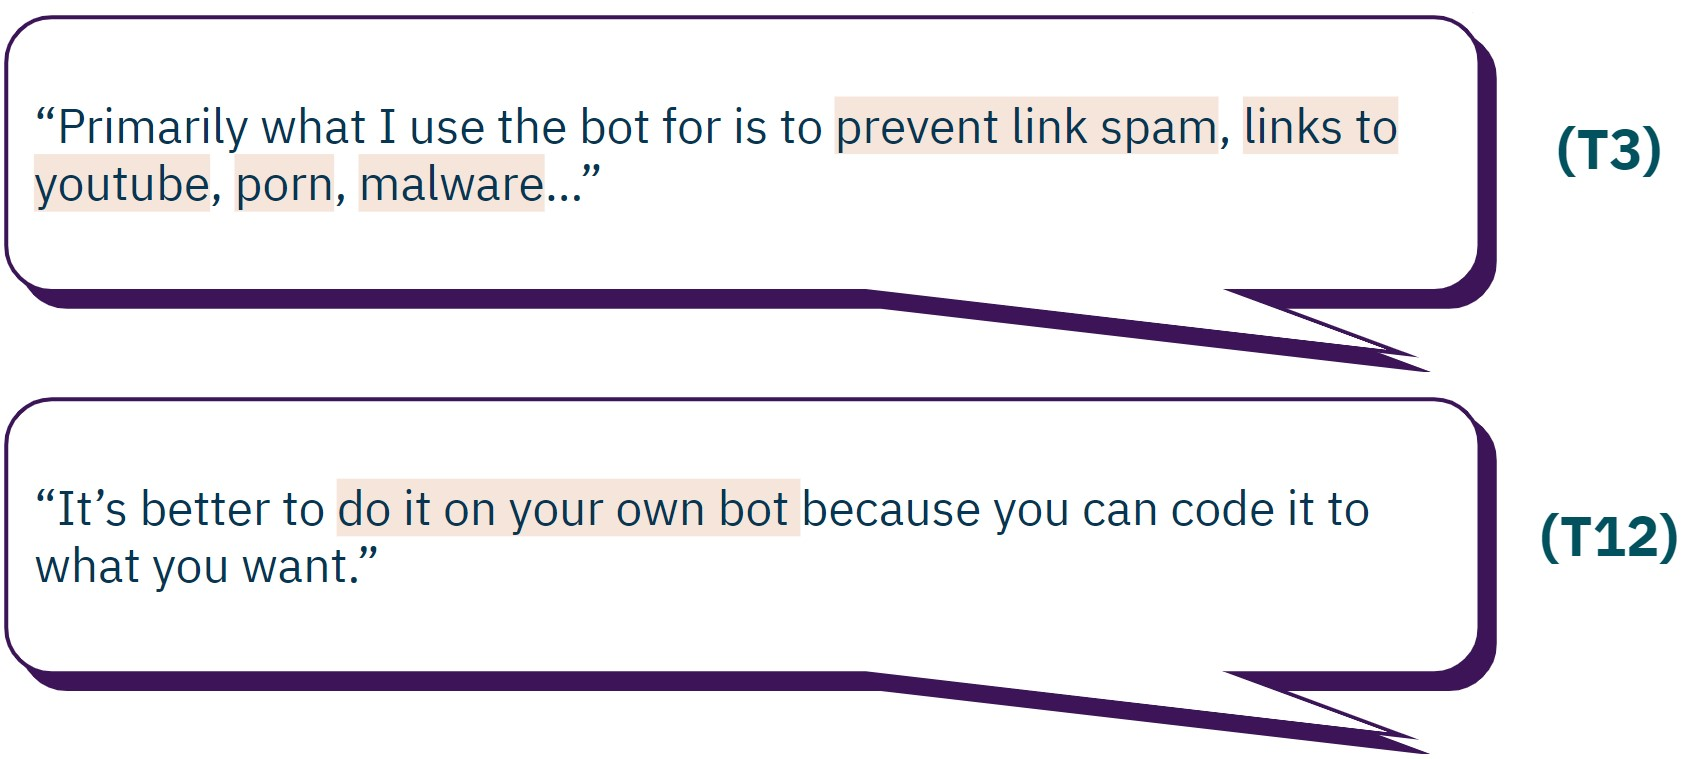
\includegraphics[width=\textwidth]{img/fig21.jpg}

\end{frame}


%%%%%%%%%%%%%%%%%%%%%%%%%%%%%%%%%%%%%%%%%%%%%%%%
%%%%%%%%%%%%%%%%  SLIDE 32  %%%%%%%%%%%%%%%%%%%%%
%%%%%%%%%%%%%%%%%%%%%%%%%%%%%%%%%%%%%%%%%%%%%%%%
\begin{frame}{}

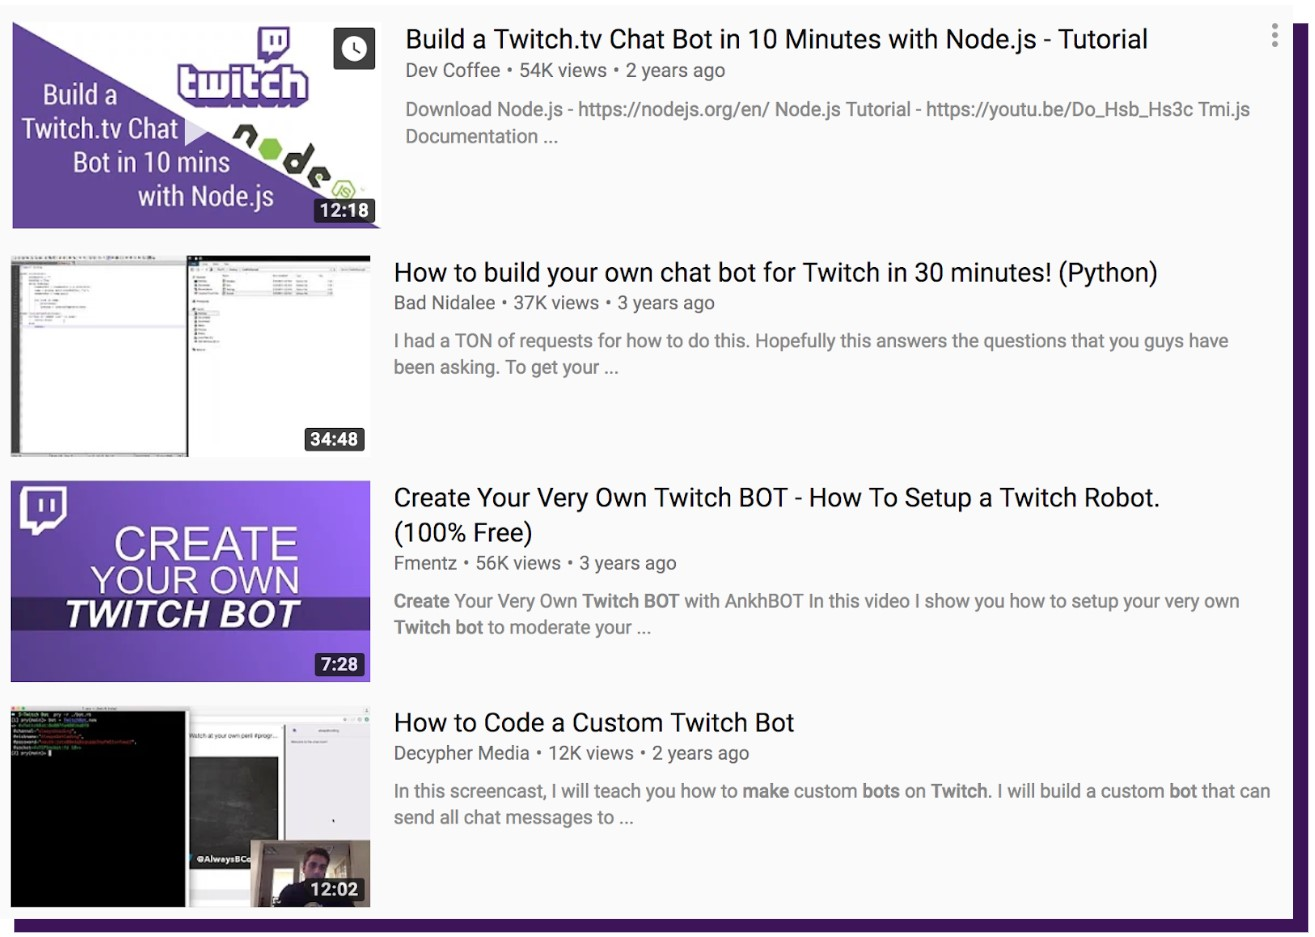
\includegraphics[width=\textwidth]{img/fig22.jpg}

\end{frame}

%%%%%%%%%%%%%%%%%%%%%%%%%%%%%%%%%%%%%%%%%%%%%%%%
%%%%%%%%%%%%%%%%  SLIDE 33  %%%%%%%%%%%%%%%%%%%%%
%%%%%%%%%%%%%%%%%%%%%%%%%%%%%%%%%%%%%%%%%%%%%%%%
\begin{frame}{Relationship with Admins}

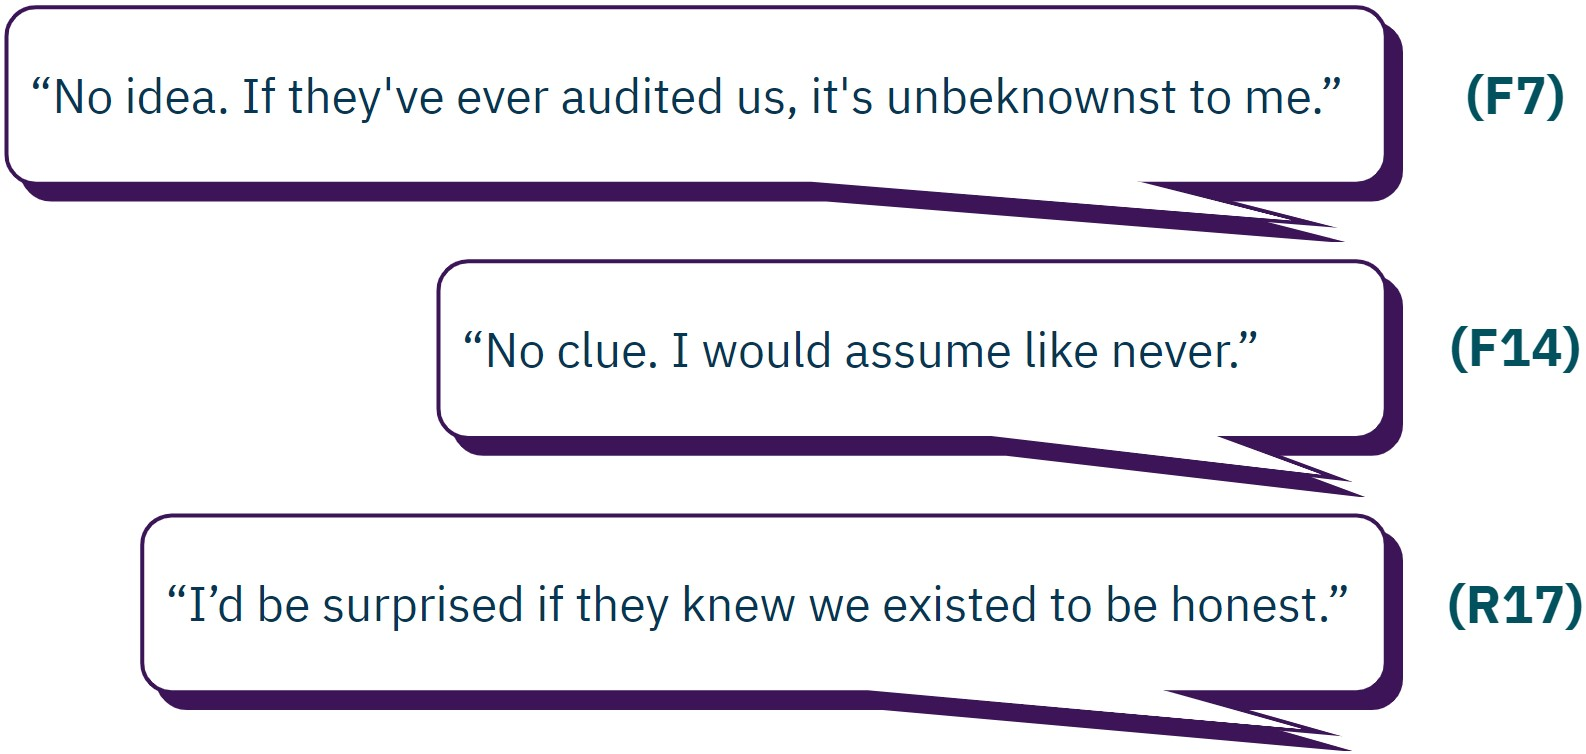
\includegraphics[width=\textwidth]{img/fig23.jpg}

\end{frame}

%%%%%%%%%%%%%%%%%%%%%%%%%%%%%%%%%%%%%%%%%%%%%%%%
%%%%%%%%%%%%%%%%  SLIDE 34  %%%%%%%%%%%%%%%%%%%%%
%%%%%%%%%%%%%%%%%%%%%%%%%%%%%%%%%%%%%%%%%%%%%%%%
\begin{frame}{}

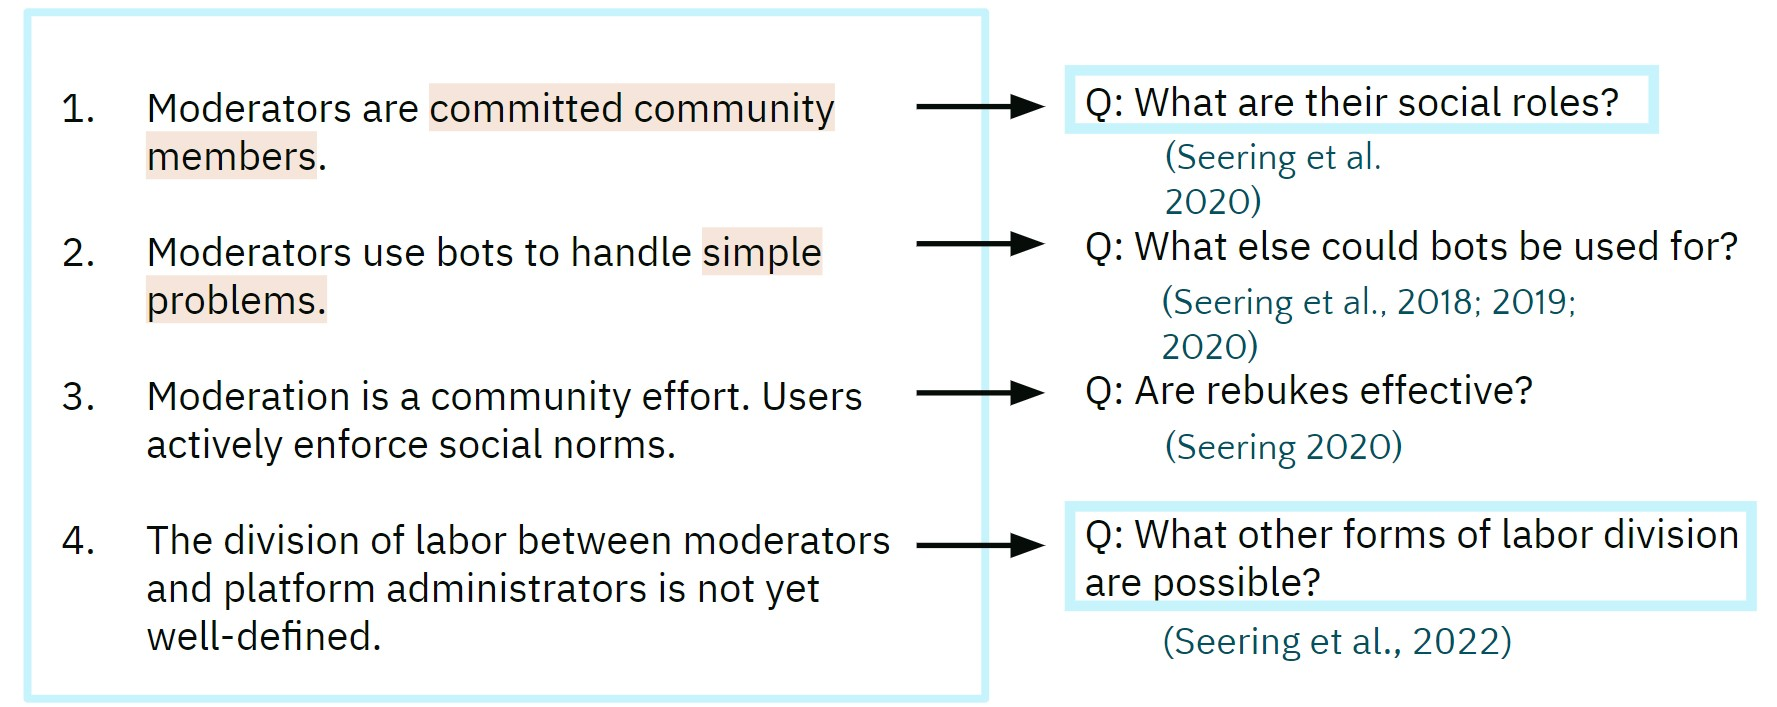
\includegraphics[width=\textwidth]{img/fig24.jpg}

\end{frame}

%%%%%%%%%%%%%%%%%%%%%%%%%%%%%%%%%%%%%%%%%%%%%%%%
%%%%%%%%%%%%%%%%  SLIDE 35  %%%%%%%%%%%%%%%%%%%%%
%%%%%%%%%%%%%%%%%%%%%%%%%%%%%%%%%%%%%%%%%%%%%%%%
\begin{frame}{Breakout task two}

People have started contributing to your wiki. There are lots of comments you have to look through to decide what’s allowed.
\newline 

With your group, \textbf{create a tab in the spreadsheet, copy the comments, and rate each comment as -1 (not okay) or 1 (okay). Copy your group’s final ratings back to the main tab.}

\note[]{Reference Disagreement Deconvolution}


\end{frame}

%%%%%%%%%%%%%%%%%%%%%%%%%%%%%%%%%%%%%%%%%%%%%%%%
%%%%%%%%%%%%%%%%  SLIDE 36  %%%%%%%%%%%%%%%%%%%%%
%%%%%%%%%%%%%%%%%%%%%%%%%%%%%%%%%%%%%%%%%%%%%%%%
\begin{frame}{}

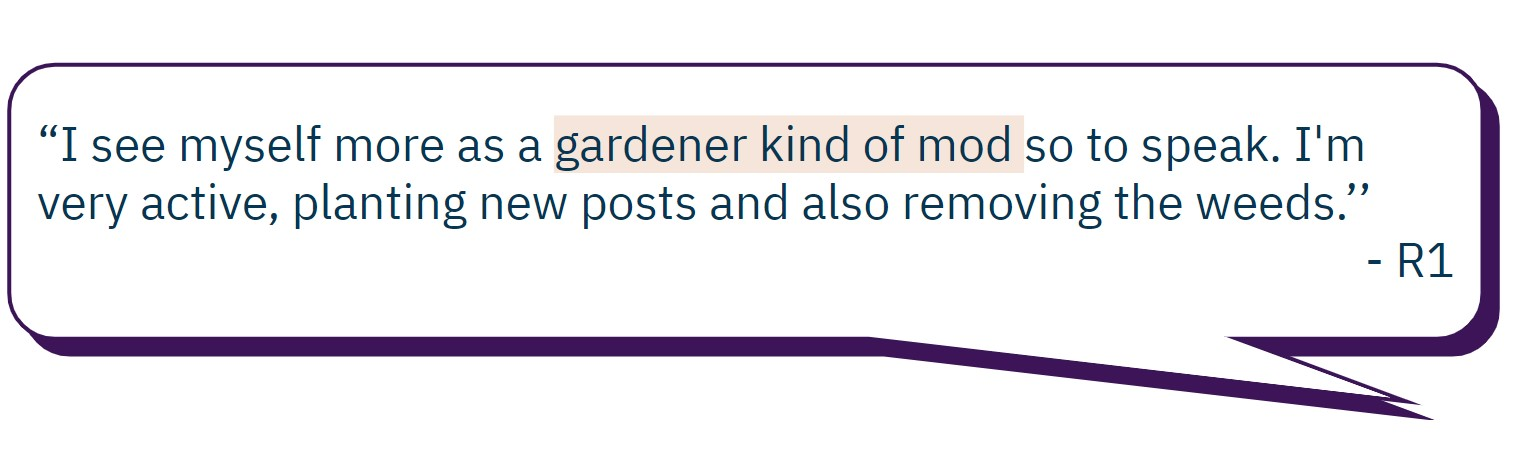
\includegraphics[width=\textwidth]{img/fig25.jpg}

\end{frame}

%%%%%%%%%%%%%%%%%%%%%%%%%%%%%%%%%%%%%%%%%%%%%%%%
%%%%%%%%%%%%%%%%  SLIDE 37  %%%%%%%%%%%%%%%%%%%%%
%%%%%%%%%%%%%%%%%%%%%%%%%%%%%%%%%%%%%%%%%%%%%%%%
\begin{frame}{}

\vspace*{3ex}
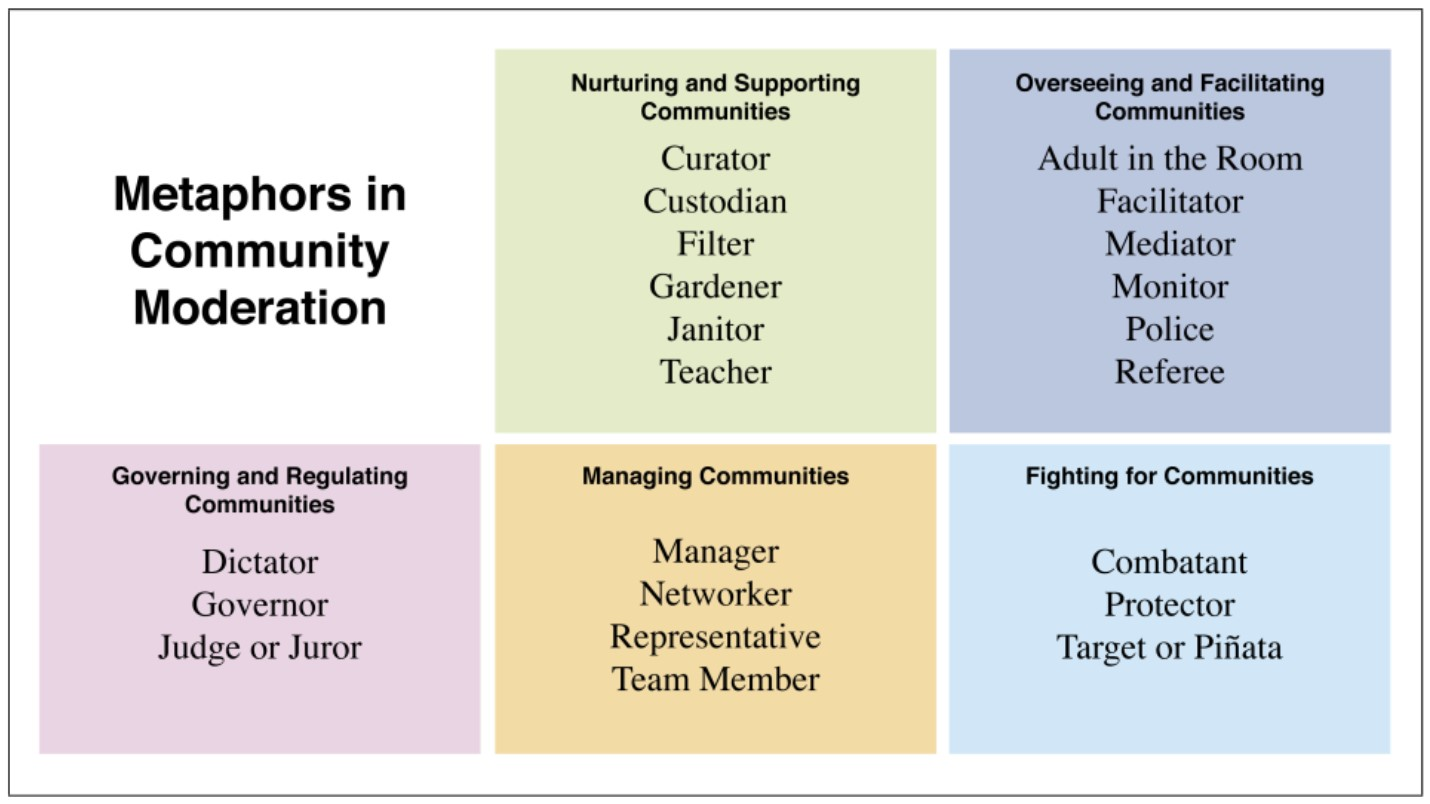
\includegraphics[width=\textwidth]{img/fig26.jpg}

\vspace{11ex}
\scriptsize{\color{lightgray}(Seering et al. 2020, “Metaphors in Moderation”)}

\end{frame}

%\backpage

\end{document}